\documentclass{sice-si}

% タイトルと著者名
\title{視覚と行動のend-to-end学習により経路追従行動を\\
オンラインで模倣する手法の提案\\
-トポロジカルマップとシナリオに基づく経路選択機能の追加と検討-\\} % 和文タイトル
\name{○春山健太(千葉工大),藤原柾(千葉工大)馬場琉生(千葉工大)\\石黒巧(千葉工大)
上田隆一(千葉工大)林原靖男(千葉工大)} % 著者名
\etitle{A proposal for an online imitation method of
path-tracking behavior by end-to-end learning of vision and action\\
- Addition and consideration  of path selection function \\based on a topological map and scenario -} % 英文タイトル
\ename{○Kenta HARUYAMA (CIT),Masaki FUJIWARA (CIT),Ryusei BABA (CIT),\\
Takumi ISHIGURO (CIT),Ryuichi UEDA (CIT),Yasuo HAYASHIBARA (CIT)}	%著者名(英)

\begin{document}
% アブストラクト
\abst{
We have proposed a method to select a route and move autonomously to a destination using camera images and target directions.
In this paper introduces an additional method for creating target directions from camera images and autonomously moving to the destination without using metric maps.
We confirmed the effectiveness of the method through the experiments using a real robot.
}

% タイトルの出力
\maketitle

% 本文
\section{緒言}
実世界では,ある特定のセンサが機能しない状況におちいり.ロボットの自律移動が継続できない場合がある.
この問題に対しては,複数の種類のセンサを用いて自己位置推定する方法や,
ナビゲーション手段自体を冗長化する方法が考えられる.
本研究グループでは,冗長化に向けて,
一般的に用いられるLiDARと地図によるナビゲーションを機械学習で模倣することで,
視覚によるナビゲーションを獲得する方法を提案した\cite{haruyama2022}\cite{fujiwara2023}.
一般的な模倣学習が人の挙動を模倣するのに対して,提案手法はLiDARと地図によるナビゲーションの
出力を模倣するため,データセットを収集する手間を省くことができるという特長がある.
さらに前報\cite{haruyama2022}\cite{fujiwara2023}では,
分岐路で指定した方向(以後,目標方向と呼ぶ)に移動する機能を追加した.
これにより,ロボットは Fig.1 のように指示された方向に移動するように,カメラ画像に基づいて経路を移動する.
ただし,前報までのシステムは,
目標方向をカメラ画像により生成していなかったため,カメラ画像のみで目的地まで移動することはできなかった.
\par
% 前報\cite{haruyama2022}\cite{fujiwara2023}ではカメラ画像に基づいて目的地まで自律移動する際に,
% Fig.\ref{fig:camera_base}のようにカメラ画像から目標方向を作成していなかった.
% そこで,カメラ画像に基づいて目標方向を作成する方法を検討する.
本稿では,カメラ画像のみで目的地に移動するために,
カメラ画像から分岐路での目標方向を生成する機能を追加する.
% カメラ画像から目標方向を作成する方法として,
具体的には,島田ら\cite{shimada2020}が提案したトポロジカルマップと「条件」や「行動」による経路の表現
(以後,シナリオと呼ぶ)をこれまで提案した手法へ追加する.
これにより,カメラ画像とトポロジカルマップから作成されるシナリオに基づいて,
目的地まで自律移動するシステムを構築する.
このシステムにより,事前に作成したメトリックマップを必要せずに,
カメラ画像を入力として目的地まで自律移動できる可能性がある.
\par
メトリックマップを用いず,カメラ画像に基づいて自律移動を行う研究はいくつかある.
Dhruvら\cite{shah2022lmnav}は大規模な事前学習モデルを用いて,自然言語による指示から,
画像によるナビゲーションをend-to-endで行う手法を提案している.
またmiyamotoら\cite{seg_meizi}はカメラ画像と深層学習による走行可能領域の検出と
トポロジカルマップを用いたナビゲーション手法を提案している.
これらの手法では,補助的ではあるが,Global Navigation Satellite System(GNSS)
やホイールオドメトリといった情報を
必要と
% することが本稿で提案する手法との違いに挙げられる.
している.センサ入力という観点で比較すると,
本システムはカメラ画像のみで目的地まで移動できるという違いがある.
本稿では,提案するシステムにより目的地までカメラ入力のみで自律移動できるかを,
実ロボットを用いた実験により検証する.
% 提案システムの有効性を実ロボットを用いた実験により検証する.
% 本稿では,カメラ画像を入力とする経路追従に対して,
% 島田らが提案した「突き当りまで」という「条件」や「直進」などの「行動」
% で表現されるシナリオ\cite{shimada2020}を
% 事前に作成したメトリックマップを用いず,
% トポロジカルマップとそこから作成されるシナリオを用いてとカメラ画像と
% 基づいてメトリックマップなしで目的地まで自律移動する手法を提案する.
% また,実ロボットを用いた実験を通して,提案した手法の有効性を検証する.
% \begin{figure}[htb
%     \centering
%      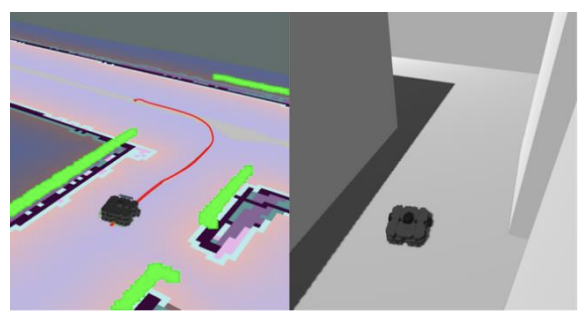
\includegraphics[height=40mm,width=80mm]{./figs/map_base.png}
%      \caption{Imitation learning of path-tracking}\label{fig:mapbase}
% \end{figure}
\begin{figure}[h]
    \centering
     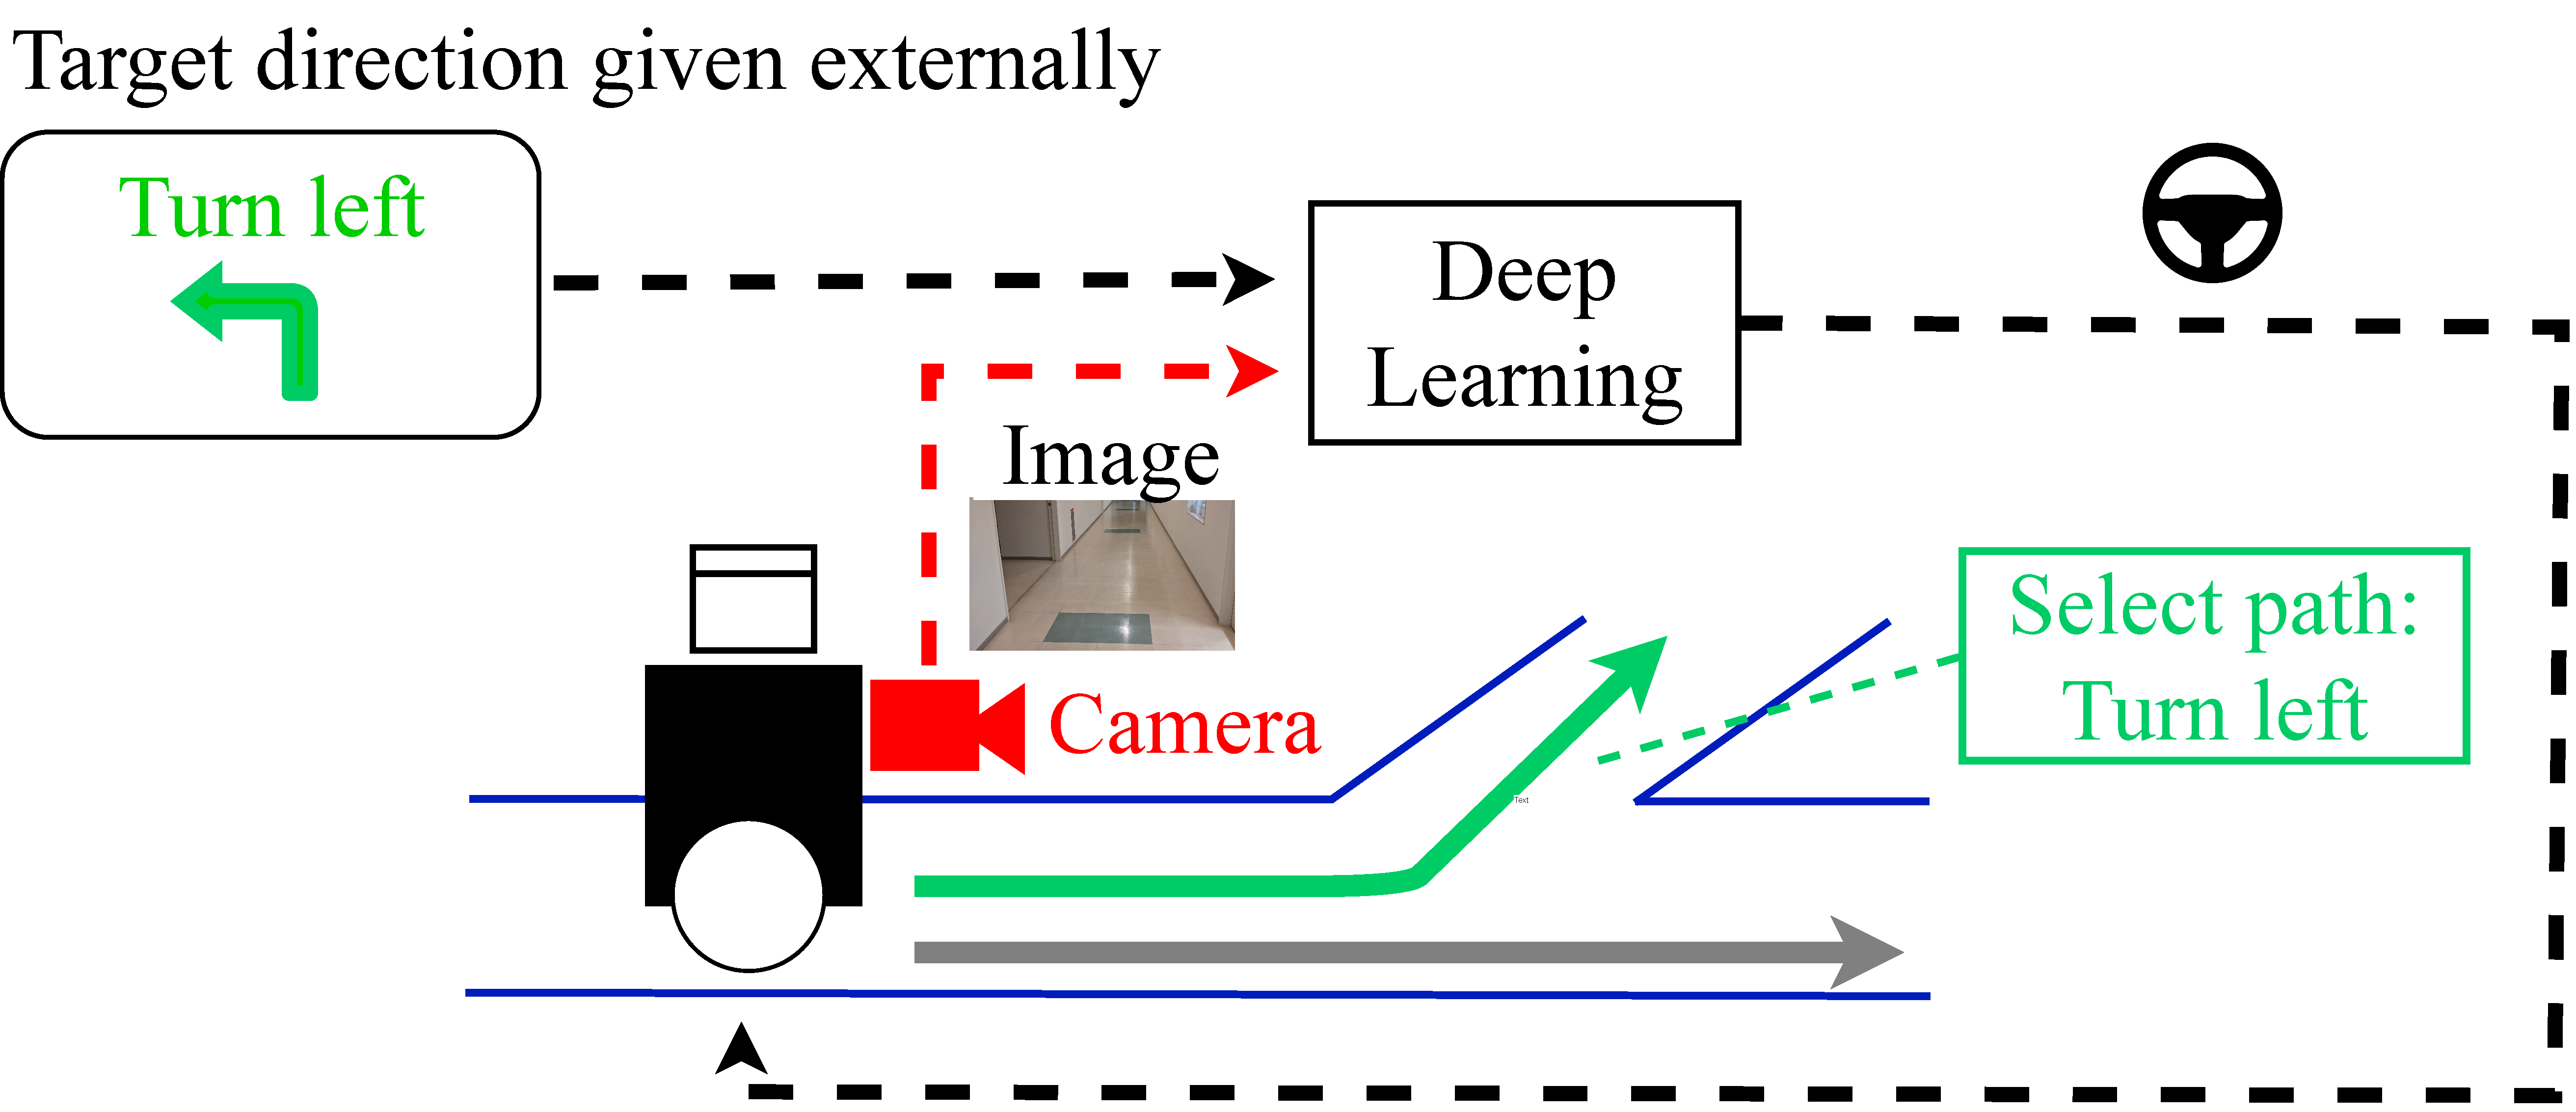
\includegraphics[height=33mm,width=78mm]{./figs/camera_base.pdf}
    %  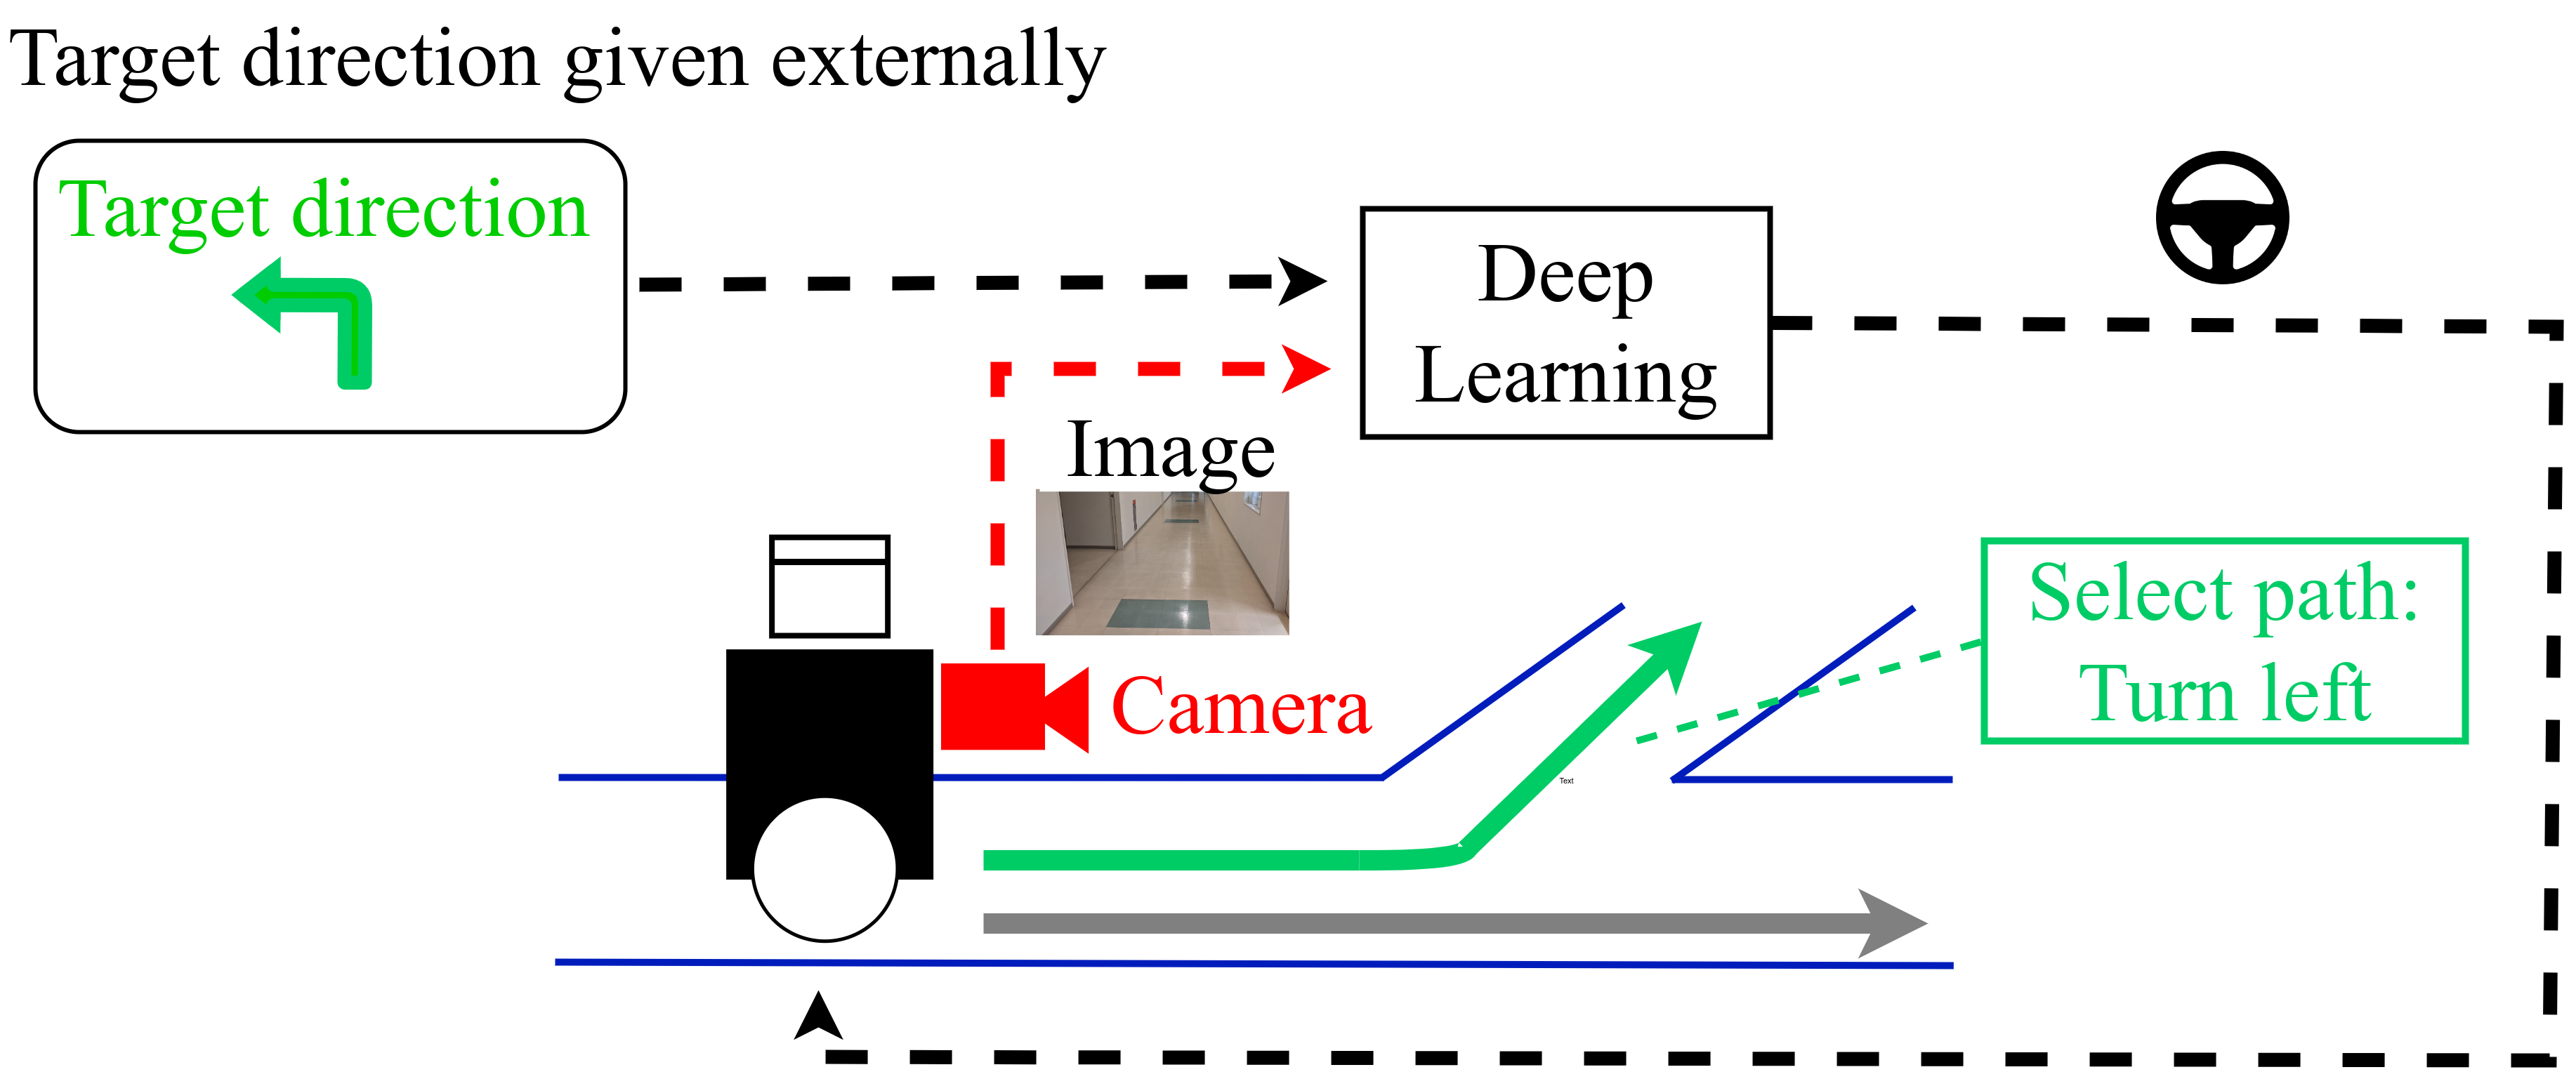
\includegraphics[height=35mm,width=78mm]{./figs/learninggamma.png}
     \caption{Path selection and following behavior based on camera images and
     target direction by imitation learning.}\label{fig:camera_base}
\end{figure}
\begin{figure*}[t]
    \centering
     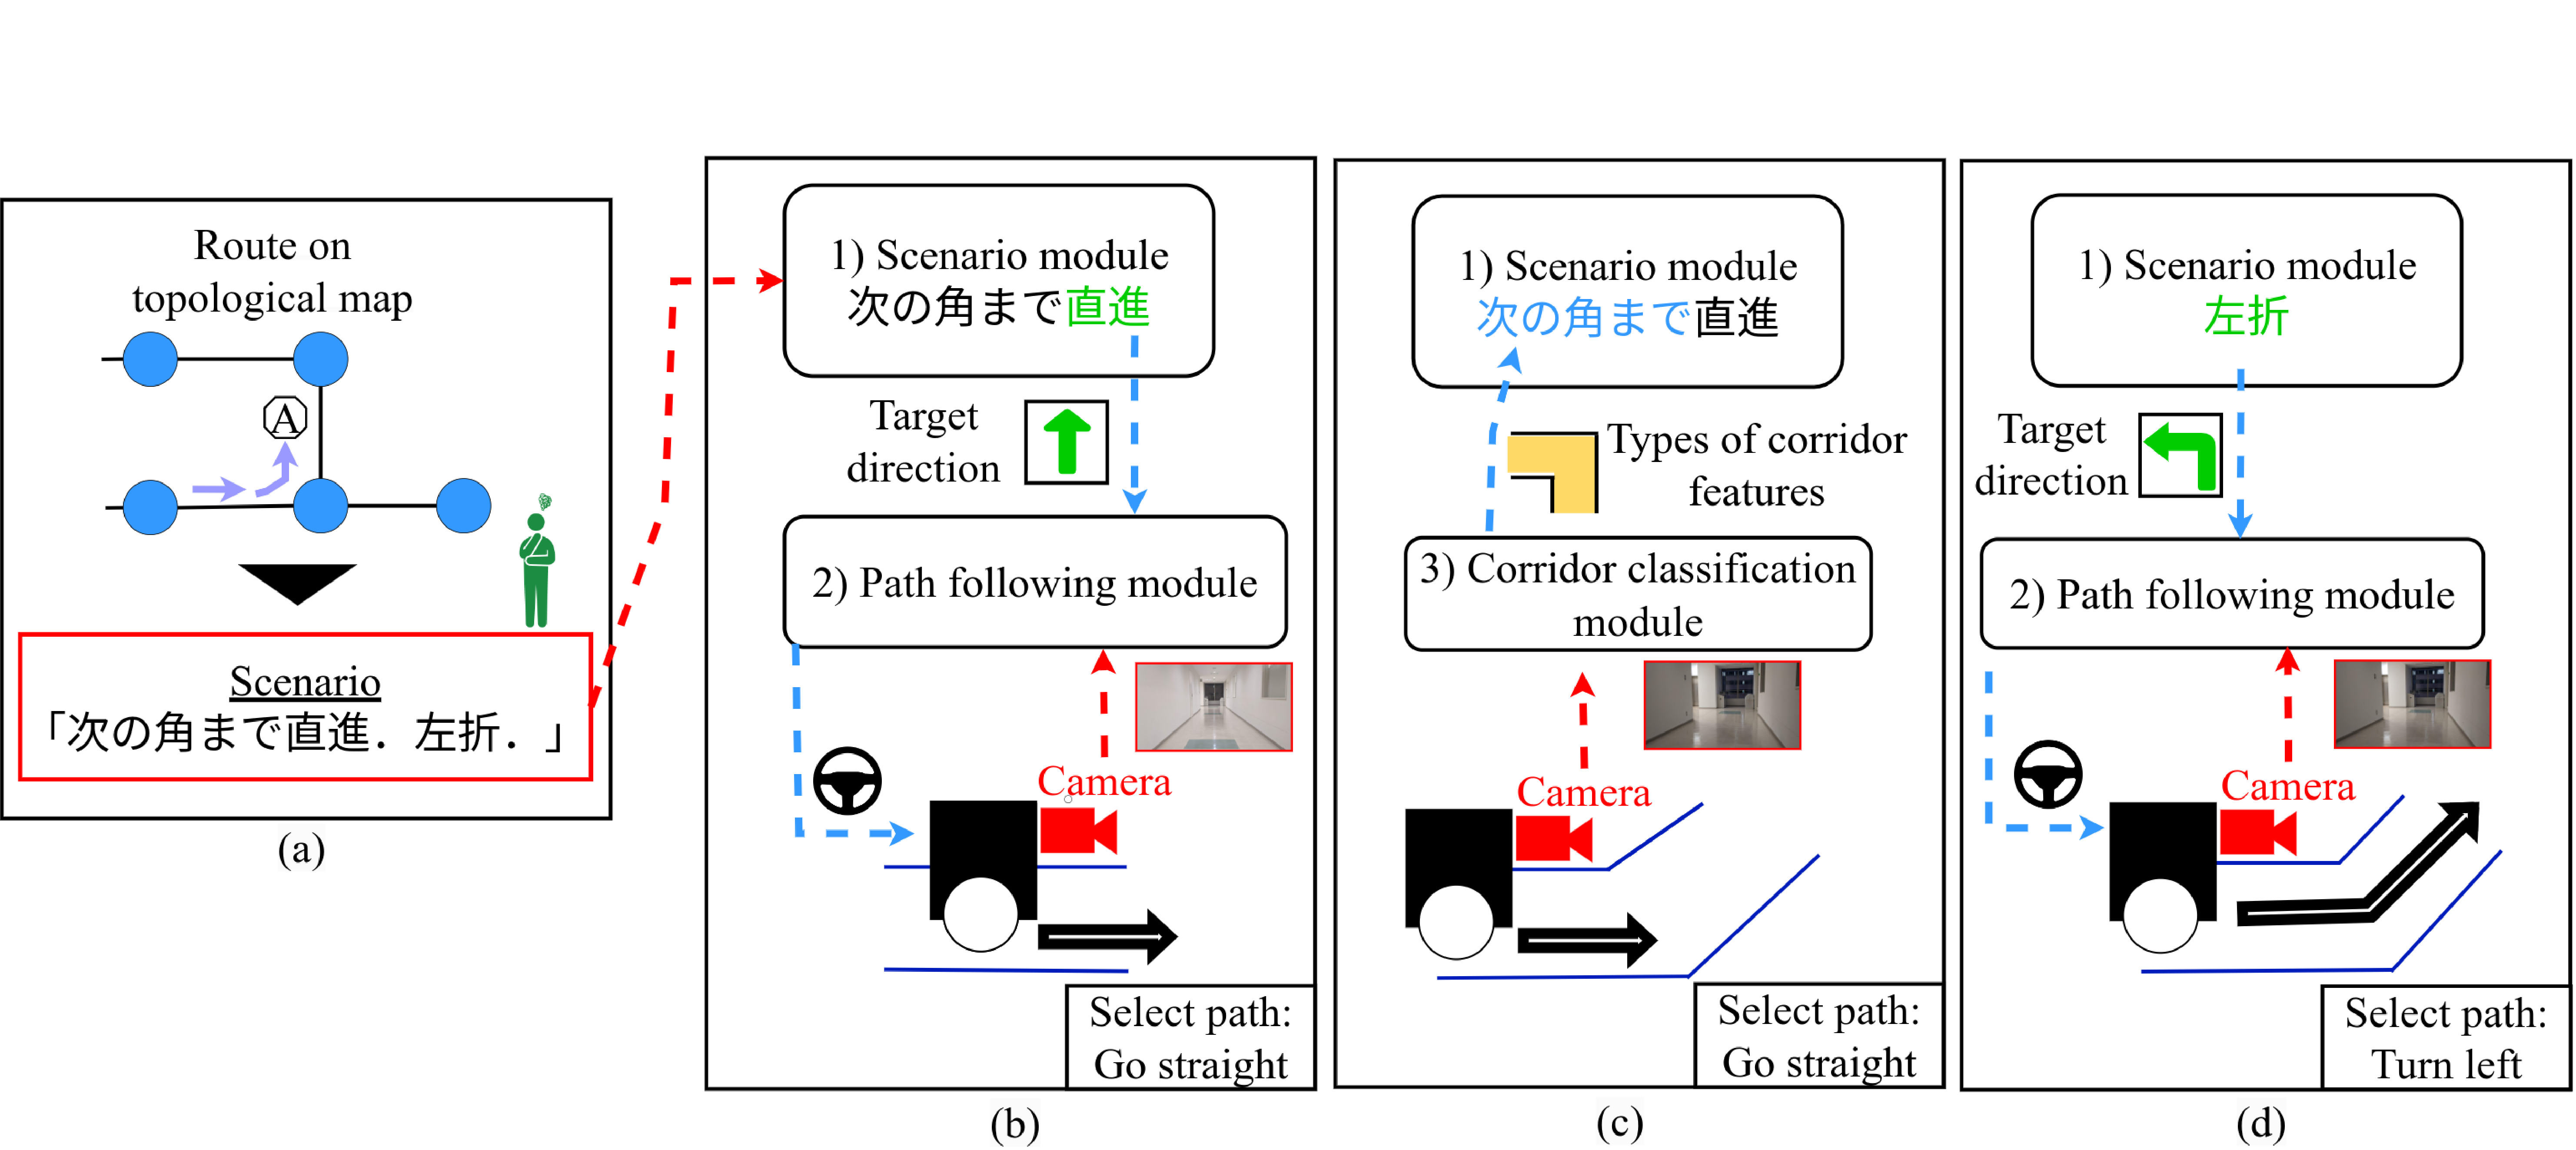
\includegraphics[height=60mm,width=160mm]{./figs/absv3.pdf}
    %  
\includegraphics[height=50mm,width=160mm]{./figs/absv3_5.pdf}
     \caption{Overview of proposed system}\label{fig:system}
\end{figure*}
\section{提案システム}
提案するシステムについて述べる.
提案するシステムでは,人間が作成した「次の角まで直進.左折.」などのシナリオから
指示された道順に従い,カメラ画像に基づいて目的地まで自律移動する.
% この手法の特徴として,目的地までの自律移動に,LiDARなどを用いて事前に
% 作成したメトリックマップを必要としないことが挙げられる.
本章ではシステムの概要について述べた後,それぞれのモジュールの詳細を述べる.
\par
Fig.\ref{fig:system}に提案システムの概要と一連の流れを示す.
提案システムは,\\
1)シナリオを分解し,「条件」と「行動」を抽出するモジュール(以後,シナリオモジュールと呼ぶ)\\
2)カメラ画像と目標方向に基づいて,経路を追従するモジュール(以後,経路追従モジュールと呼ぶ)\\
3)カメラ画像を基に通路の特徴を分類するモジュール(以後,通路分類モジュールと呼ぶ)\\
の3つのモジュールで構成される.
% はじめに,人間が作成したシナリオがモジュールへ入力される.
% 自律移動時はロボットに取り付けたカメラから得た画像データを入力とする
% システムは,ロボットに取り付けたカメラから得た画像データと,
% トポロジカルマップを基に人間が作成したシナリオを入力とし,
% \begin{enumerate}
%     \item [1)] シナリオの条件を満たしたかの判定に用いる,通路の特徴を分類する通路分類モジュール
%     \item [2)] シナリオを解釈し,目標方向へ変換して出力するモジュール
%     \item [3)] カメラ画像と目標方向に基づく経路追従モジュール\
% \end{enumerate}
ロボットは下記のaからdの一連の流れにより,
指示された経路に沿って目的地まで自律移動する
\begin{enumerate}
    \item [(a)] トポロジカルマップ上の目的地に応じて,
    人間が「条件」と「行動」で構成されるシナリオを作成する.
    例えば,図のAを目的地とするシナリオは「次の角まで直進.左折.」となる.
    \item [(b)] 作成したシナリオをシナリオモジュールへ入力する.
    シナリオモジュールは入力されたシナリオを分解し,「条件」と「行動」を抽出する.
    1つ目の条件と行動のセットは「次の角まで」と「直進」となる.
    この「直進」を目標方向として経路追従モジュールへ与える.
    経路追従モジュールは,カメラ画像と与えられた
    目標方向に基づいて,経路に沿って直進する.
    \item [(c)] ロボットが角に近づくと,
    % 通路分類モジュールの分類結果が角となり,
    通路分類モジュールがカメラ画像に基づいて
    通路を「角」と分類して,それをシナリオモジュールに与える.
    シナリオモジュールはそれを基に「次の角まで」という条件を満たしたかを判定する.
    この場合は条件を満たしているため,2つ目の行動である「左折」
    へ遷移する.
    \item [(d)]「左折」に基づいて,経路追従モジュールは
    経路に沿って角を左折する.
\end{enumerate}
% Fig.\ref{fig:system}(a)でトポロジカルマップとこのマップ上の経路から
% 人間が「条件」と「行動」で構成したシナリオを作成する.
% ここで作成されるシナリオは「次の角まで直進.右折.」となる.
% Fig.\ref{fig:system}(b)では,作成されたシナリオを1)の
% シナリオを解釈するモジュールが分解し,「次の角まで直進」が抽出される.

% この入力されたシナリオを2)のモジュールが「条件」と「行動」に分解し,
% この行動を目標方向へ変換して出力する.
% 具体的には,1)の通路分類モジュールから「三叉路」という分類結果が得られるまで,
% 「直進」の目標方向を出力し,3)の経路追従モジュールへ与える.
% 3)の経路追従モジュールはカメラ画像と与えられた目標方向をもとに,
% 「直進」の経路を追従する.
% 1)の通路分類モジュールから「三叉路」の分類結果が得られた場合,
% 2)のモジュールは次に「右折」の目標方向を出力し,
% 3)のモジュールは経路に沿って右折する.


\subsection{経路追従モジュール}
% カメラ画像と目標方向に基づいて,
前報[1][2]の提案手法に基づき構築した経路追従モジュールについて述べる.
このモジュールは,事前に模倣学習させた環境で,
カメラ画像に基づいて経路を追従するモジュールであり,
分岐路では入力された目標方向によって経路を選択して走行する.
% カメラ画像に基づく経路追従は,
% メトリックマップを用いたルールベース制御器の出力を模倣するように学習することで
% 獲得する\cite{haruyama2022}\cite{fujiwara2023}.
% これにより,学習後はRGBカメラのセンサ入力のみで経路追従が可能である.
\par
Fig.\ref{fig:learning}に経路追従モジュールのシステムを示す.
学習時は,2D-LiDARやオドメトリ,事前に作成したメトリックマップに
基づいたルールベース制御器(ROS Navigation Stack\cite{ros-navigation})によって,
設定した経路を走行する.
その際,入力をカメラ画像と目標方向,
出力をヨー方向の角速度とするデータを,0.2秒周期でデータセットに加える.
このヨー方向の角速度はメトリックマップに基づいたルールベース制御器が出力する信号である.
さらに,バッチサイズを8として教師データを抽出し,
0.2秒の周期でオンラインで学習する.
このデータセットへのデータの追加から学習までの1連の流れを1ステップとする.
学習時のデータセットへ加える目標方向には,
メトリックマップに基づいたルールベースの制御器から出力を用いる.
データセットの収集には,藤原ら\cite{fujiwara2023}が提案した
データセットの不均衡の改善,
学習時における積極的な蛇行といった最も経路追従の成功率の高い手法を採用する.
\par
学習後,モジュールはカメラ画像と目標方向を基に,
ヨー方向の角速度を出力する.
これにより経路を追従する.
このとき,並進速度は0.2m/sである.
なお,目標方向が「停止」の場合は,0.0m/sとなる.
% 並進速度には0.2m/sの一定の値を与える.
\begin{figure}[htbp]
    \centering
    %  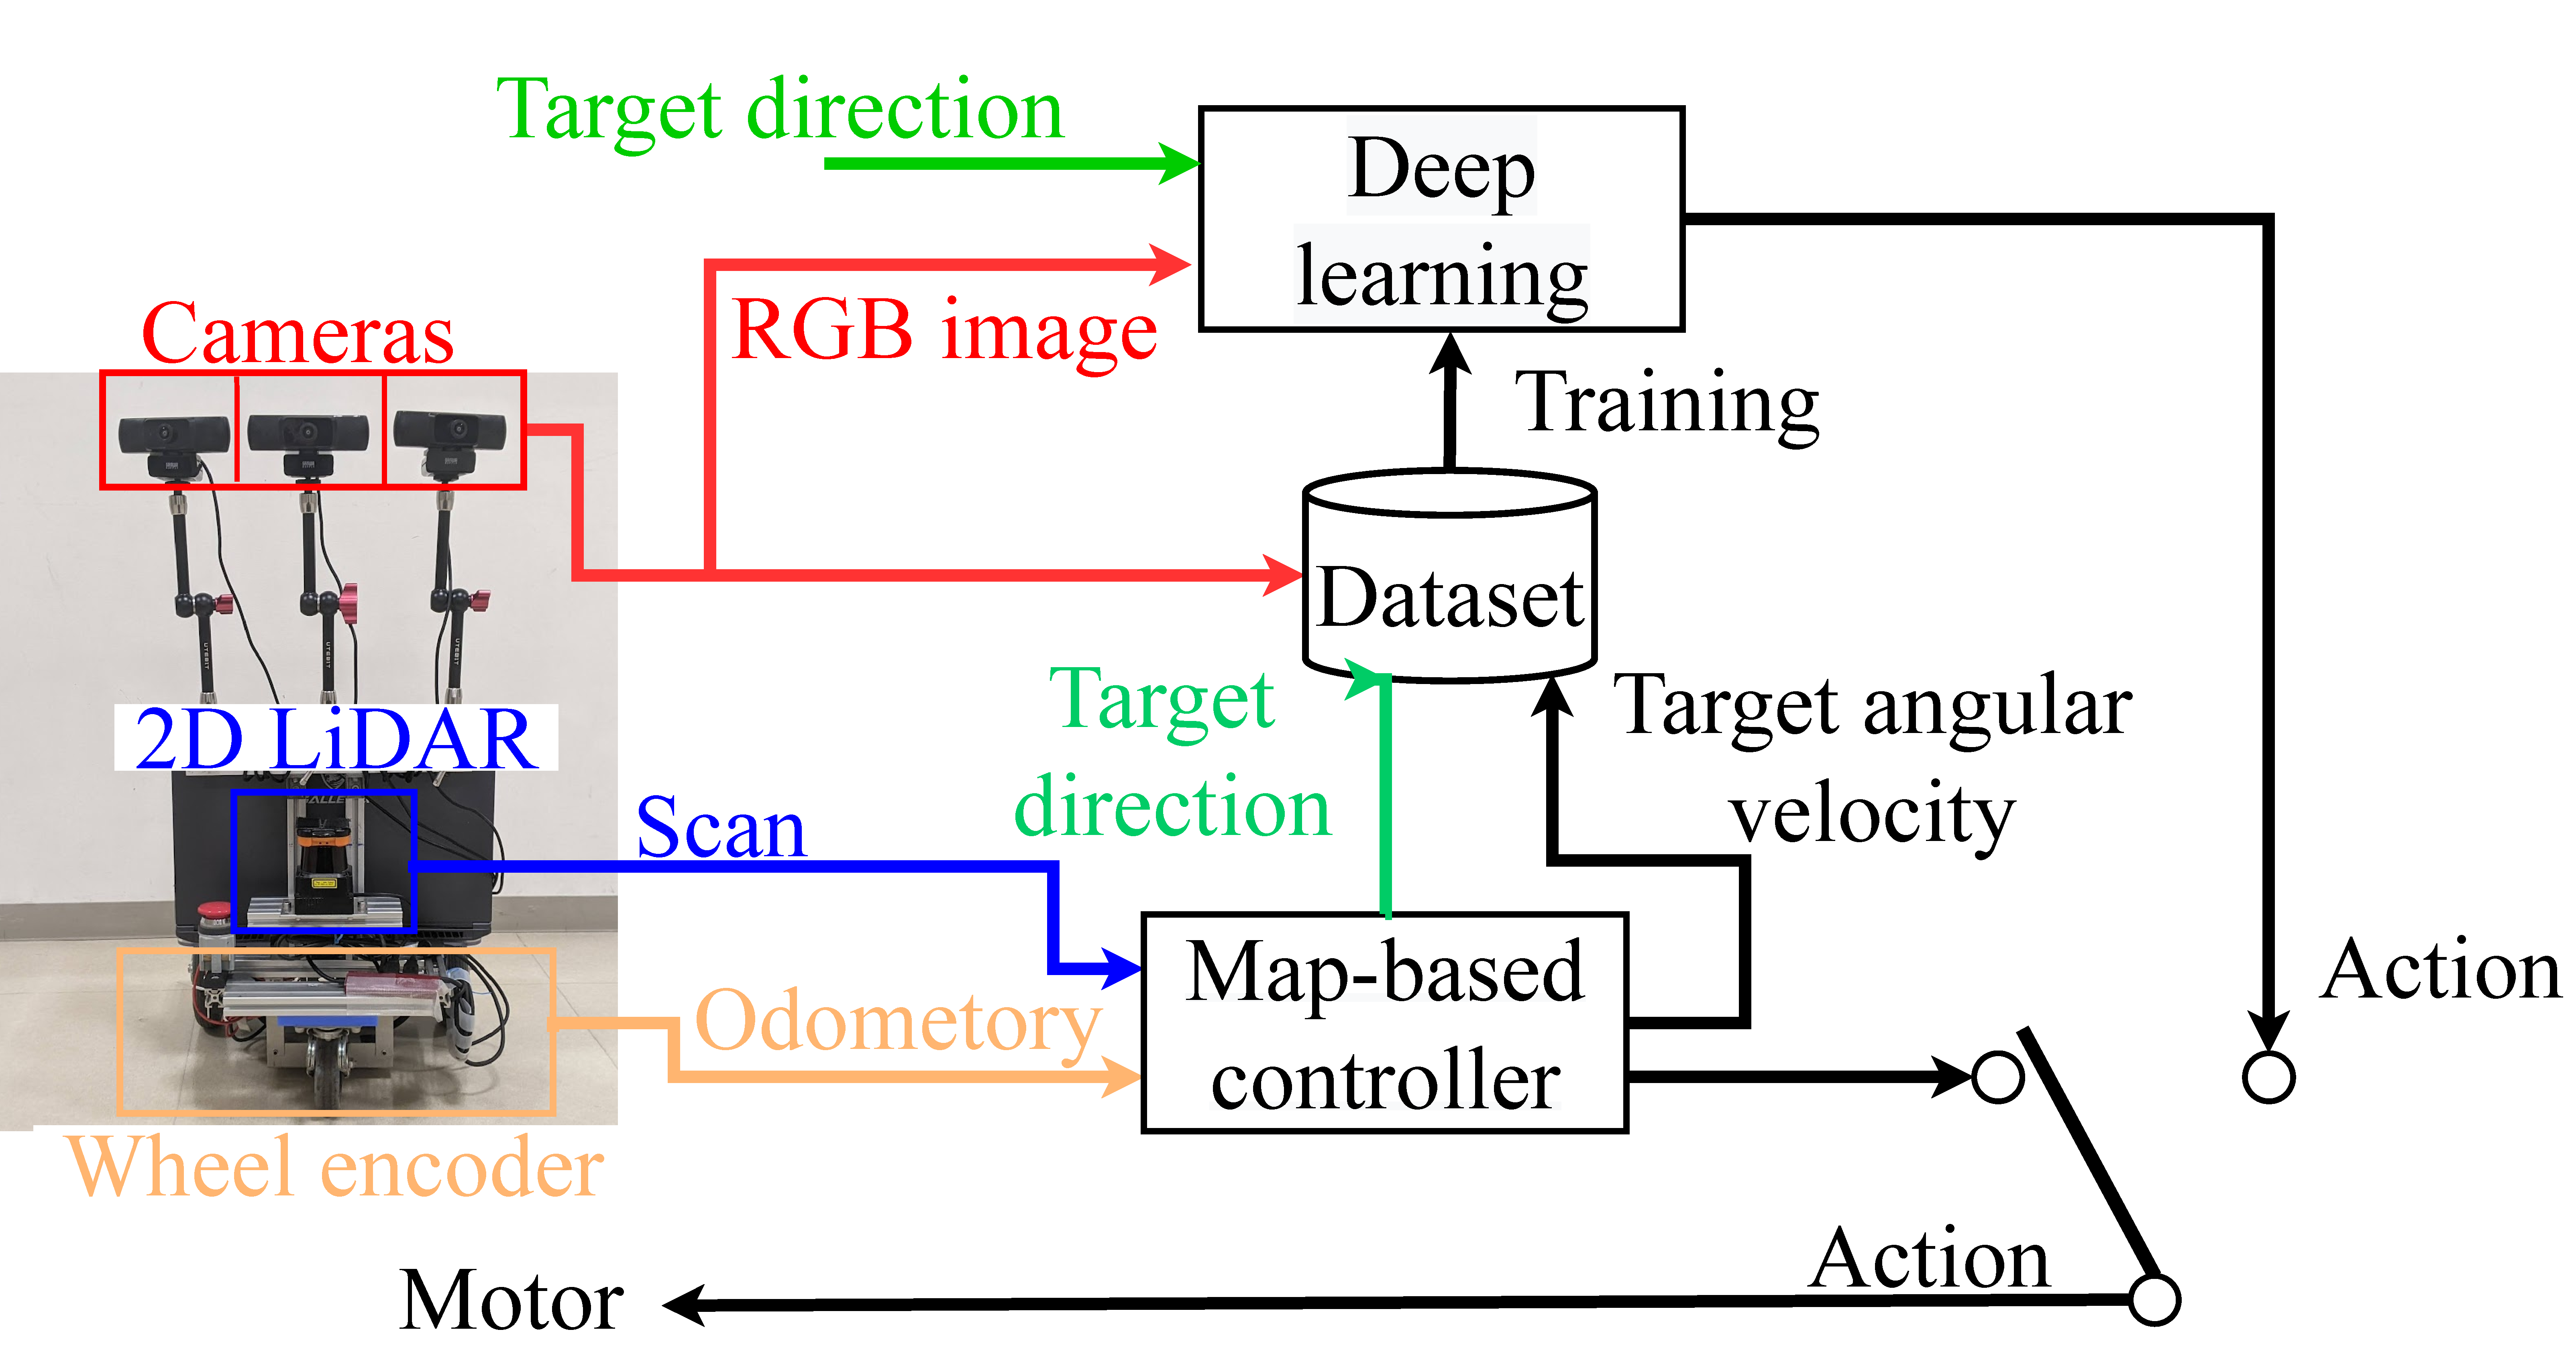
\includegraphics[height=45mm,width=80mm]{./figs/system_learning.pdf}
     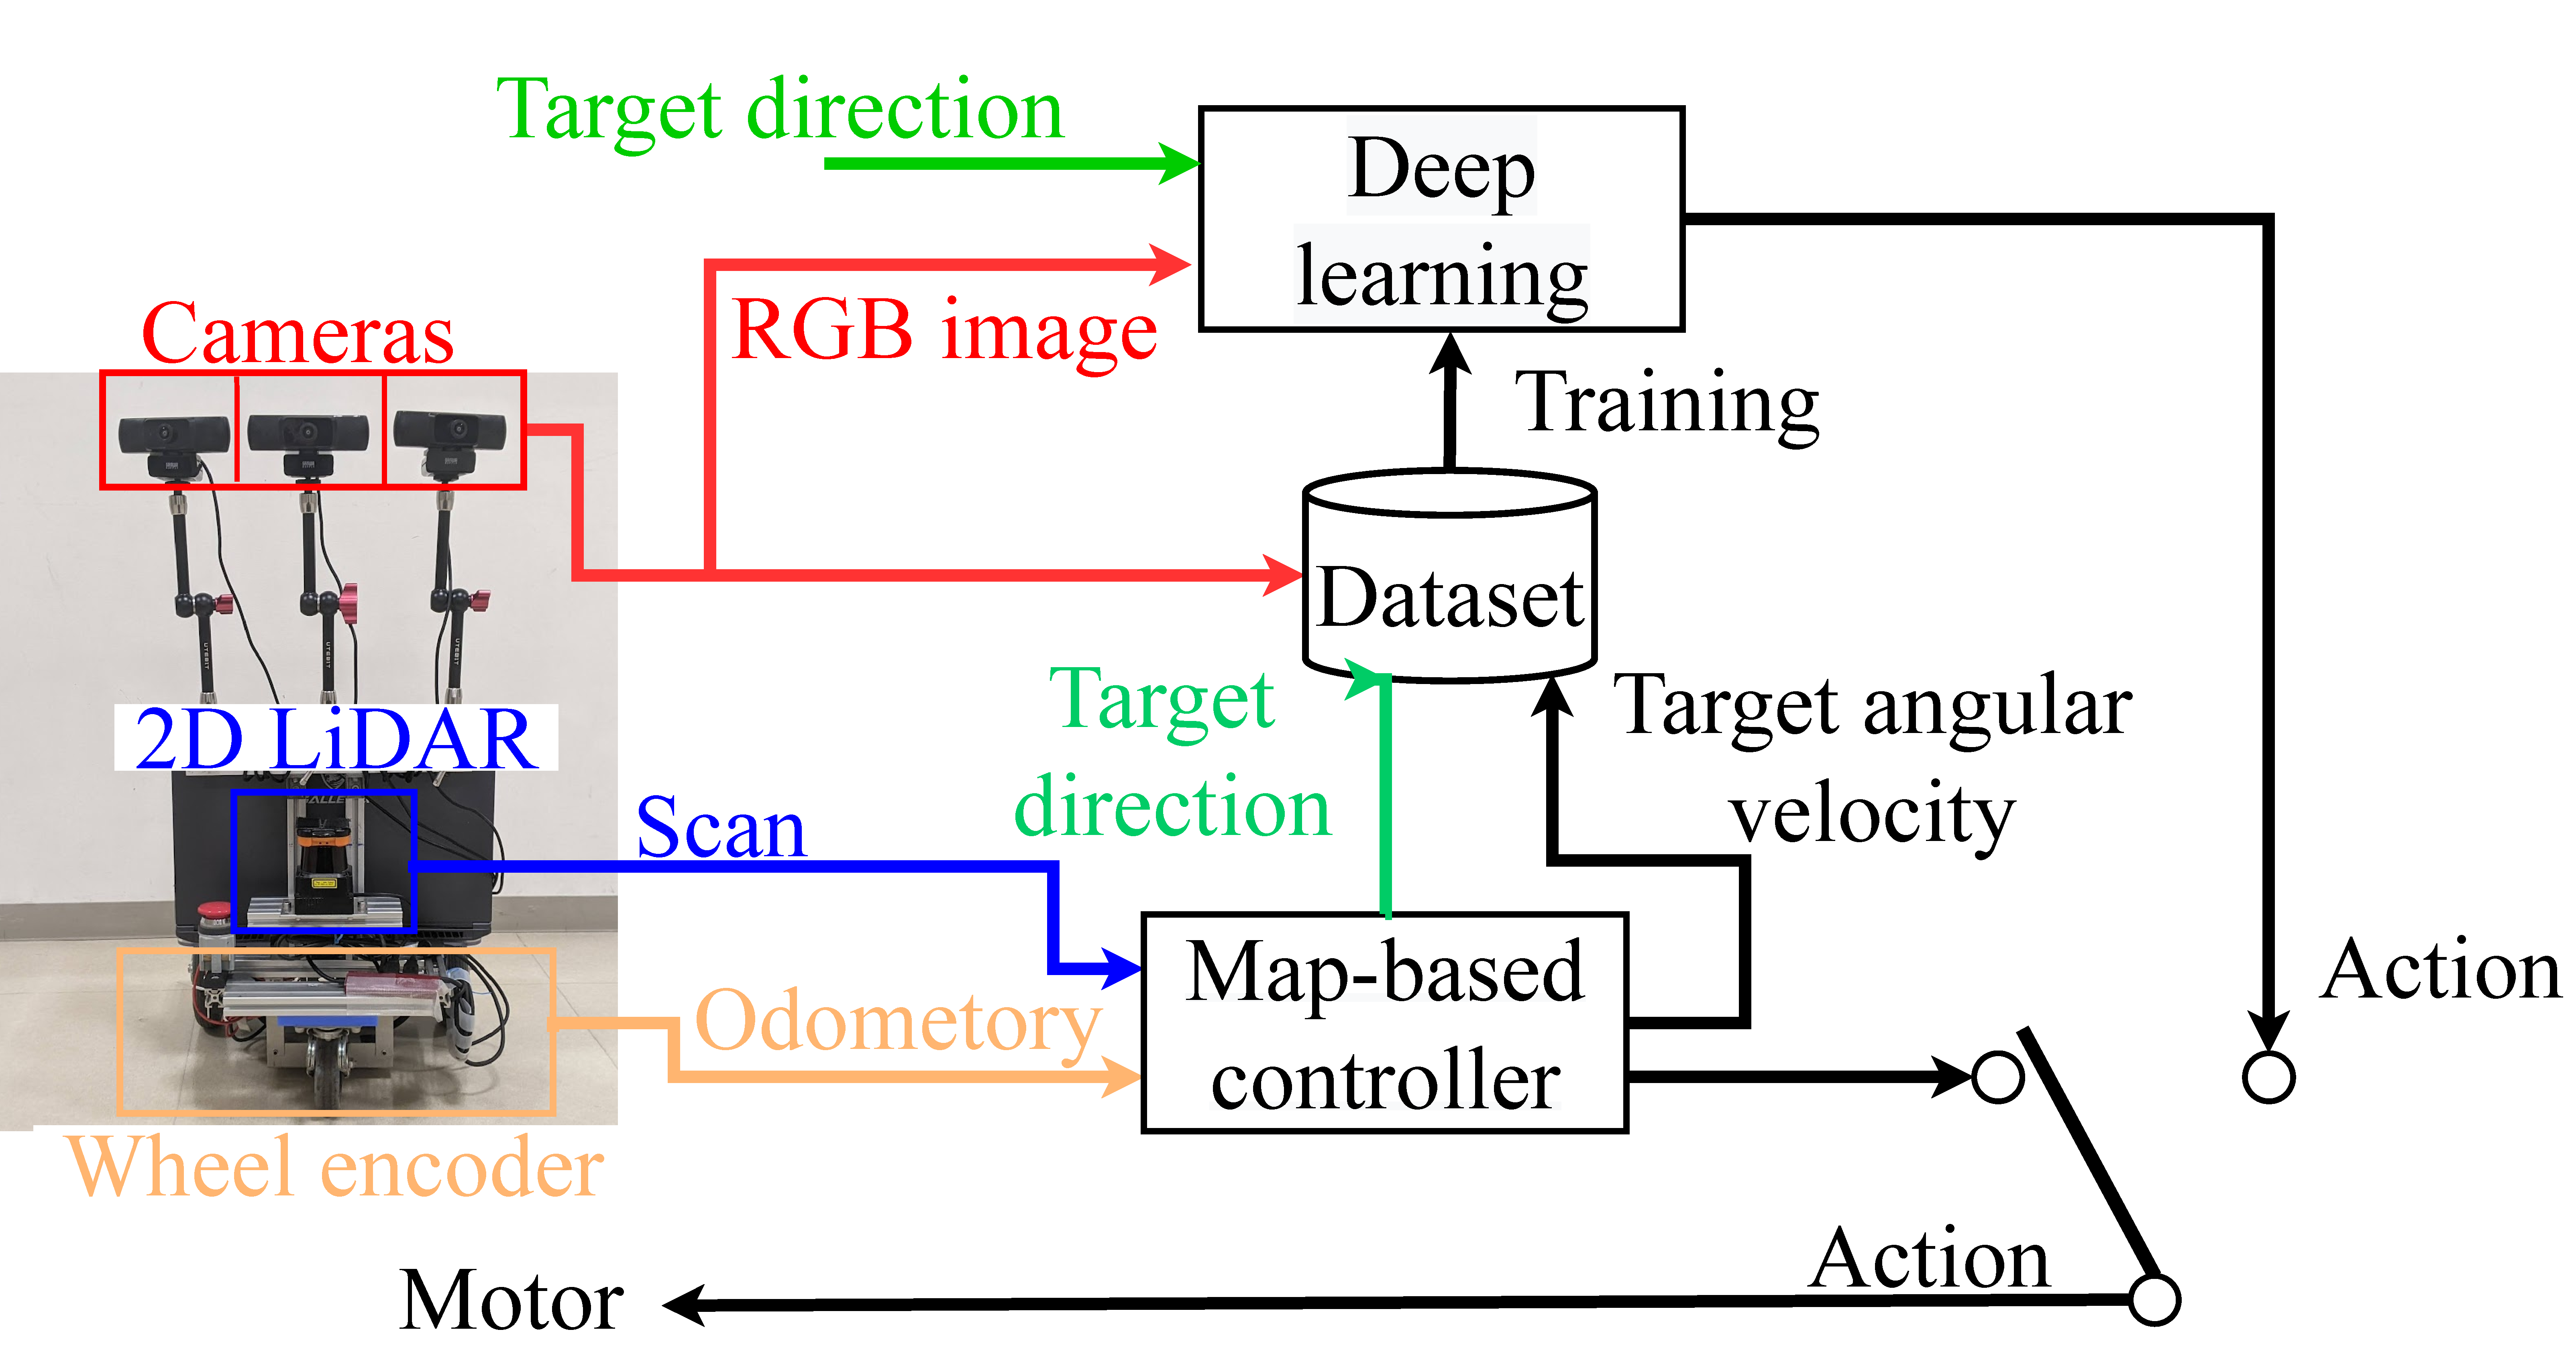
\includegraphics[width=80mm]{./figs/system_learning.pdf}
     \caption{Path-following module system}\label{fig:learning}
\end{figure}
\subsection{シナリオモジュール}
シナリオ
% から経路追従モジュールが必要とする目標方向を出力する
モジュールについて述べる.
シナリオモジュールはトポロジカルマップから作成された
シナリオから「突き当りまで」という「条件」や
「左折」などの「行動」を解釈し,単語で構成された経路を分岐路での目標方向へ変換して出力する.
% 後述する分類モジュールと組み合わせることで,目的地までの自律移動に必要な分岐路での目標方向を,
% 経路追従モジュールへ与えることを可能とする.
\par
Fig.\ref{fig:topo2sce}にトポロジカルマップの例とそれを基に作成されるシナリオを示す.
トポロジカルマップは図中の青の通路の特徴的な箇所に配置されたノード,
これらをつなぐ図中の緑のエッジで構成される.
ノードはID,通路の特徴,接続されるエッジとその方向のデータが含まれ,
エッジにはIDのデータのみが含まれている.
シナリオはトポロジカルマップ上での目的地までの経路を,「条件」と「行動」に関する単語を組み
合わせることで表現したものである.
図の例では出発地点をエッジ2,目的地をノード2として,その間のエッジとノードを移動する.
エッジ2からノード1は「三叉路まで」という条件と「直進」という行動,
ノード1からエッジ1は「右折」という行動,
エッジ1からノード2は「突き当り(三叉路)まで」という条件と「直進」の行動で表現される.
これらを統合すると,
最終的に「三叉路まで直進.右折.突き当たりまで直進.停止.」
のシナリオが作成される.\par
次に作成されたシナリオを目標方向として変換する方法を述べる.
目標方向への変換では
シナリオを句点ごとに分解後,「条件」と「行動」を示す言葉を抽出し,
以下の項目に分けて登録する.\\
% \begin{enumerate}
%     \item [1)] 通路の特徴
%     \item [2)] 順番
%     \item [3)] 方向
%     \item [3)] 方向
% \end{enumerate}
1)通路の特徴 例えば,「三叉路」「角」など\\
2)順番 例えば,「3つ目の」「2番目の」など\\
3)方向 例えば,「左手に」「右手に」など\\
4)行動 例えば,「右折」「停止」など\\
先に示した例は句点ごとに
三叉路まで直進/ 
右折/ 
突き当たりまで直進/ 
停止/ 
と分解される.
1つ目の条件と行動は
1)通路の特徴 三叉路,4)行動 直進となる.
2つ目の行動は4)行動 右折となる.
この一連の処理を末尾まで行う.
この「行動」を分岐路での目標方向に変換して,前述の経路追従モジュールへ与える.
目標方向のデータ形式をTable \ref{tab:target}に示す.
ここで,「三叉路まで」といった条件を満たしたかの判定は,後述する通路分類モジュールを用いて行う.
\begin{figure}[htbp]
    \centering
     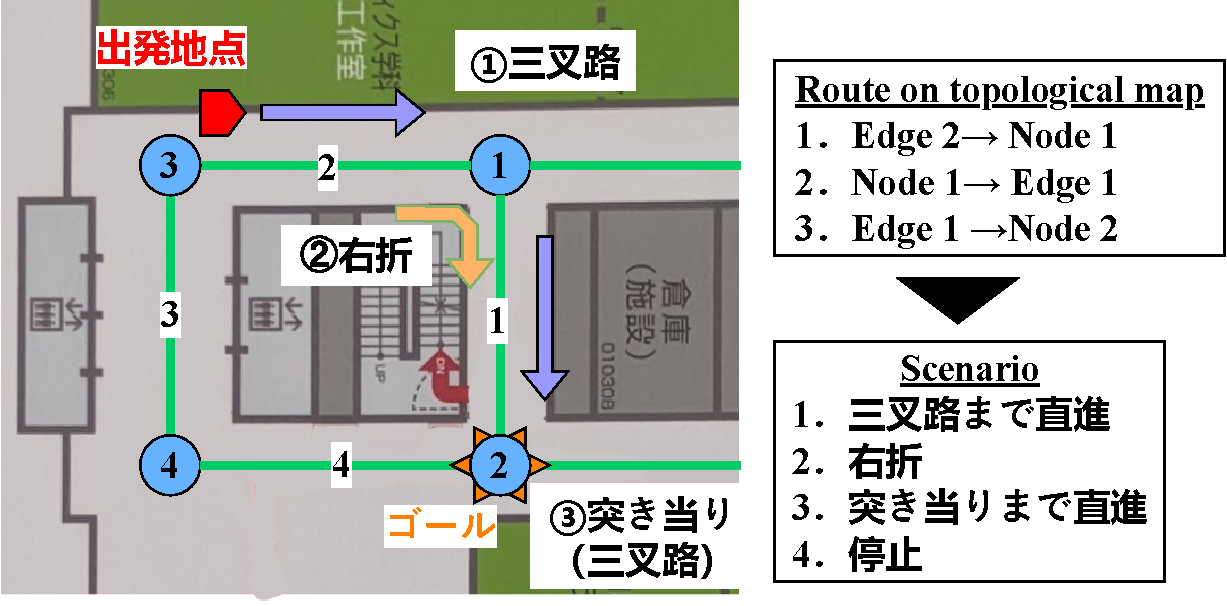
\includegraphics[height=40mm,width=80mm]{./figs/topo2sce.pdf}
     \caption{Example of topological map and created scenario}\label{fig:topo2sce}
\end{figure}
\begin{table}[]
    \centering
    \caption{Target direction and data for path-following module}\label{tab:target}
    \begin{tabular}{|c|c|}
    \hline
    Target direction & Data        \\
    \hline
    Go straight   & {[}1,0,0{]} \\
    Turn left   & {[}0,1,0{]} \\
    Turn right   & {[}0,0,1{]} \\
    Stop   & {[}0,0,0{]}\\
    \hline
    \end{tabular}
    \end{table}

\subsection{通路分類モジュール}
通路分類モジュールについて述べる.
このモジュールは,
シナリオの「条件」を満たすかの判定に必要な通路の特徴を,
カメラ画像を入力として分類する.
通路分類モジュールの概要をFig.\ref{fig:lrcn}に示す.このモジュールは
フレーム数16,画像サイズ64×48の連続した画像データ
を入力とし,通路の特徴を分類した結果を出力する.
通路の特徴の分類は島田らの手法\cite{shimada2020}に倣い,
Fig.\ref{fig:intersection}に示した8つとする.
このモジュールのネットワークアーキテクチャは
Dhaivatらが提案するCNNとLSTMを組み合わせたIntersectNet\cite{lrcn}に倣って構築した.
なお,CNNアーキテクチャにはMobileNetV3-Large\cite{v3}を用いている.
% シーケンスデータのフレーム数は16 

\begin{figure}[h!]
    \centering
    %  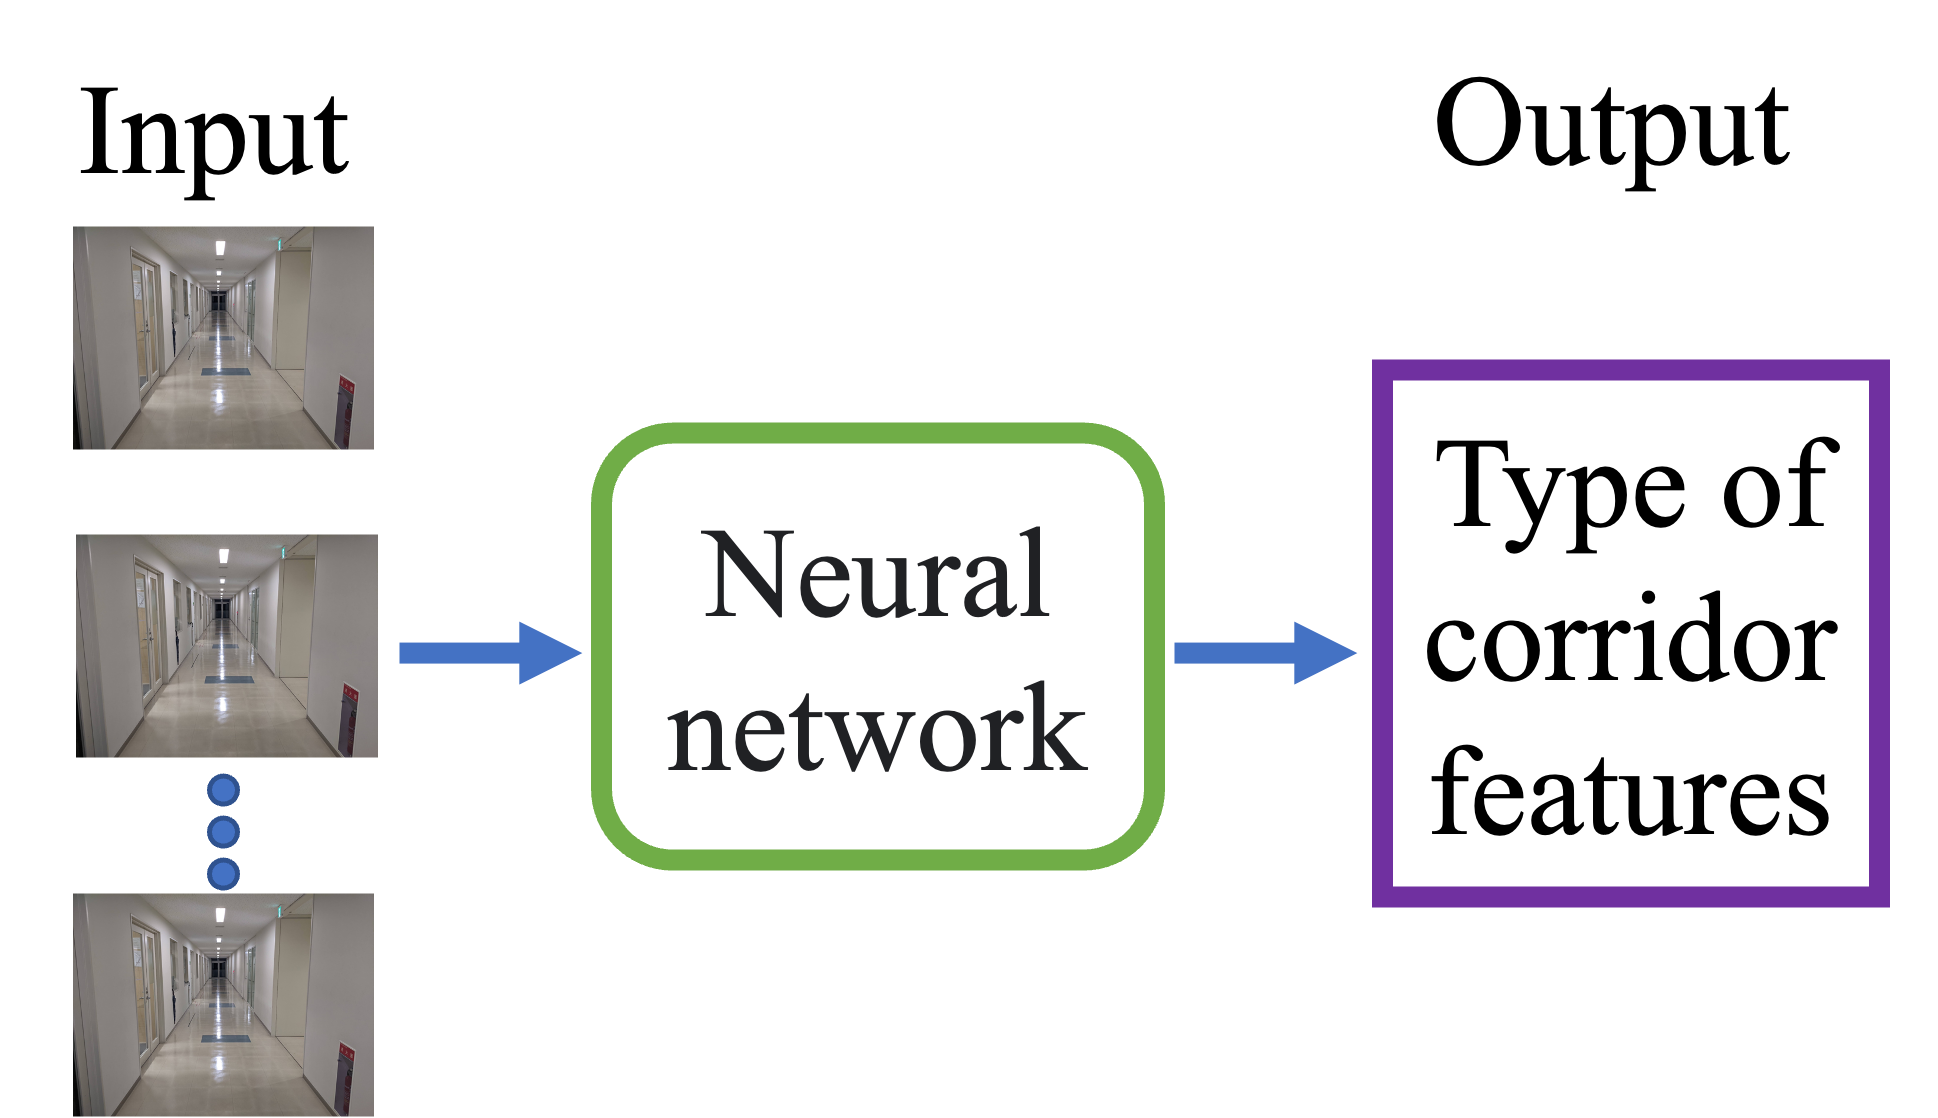
\includegraphics[height=30mm,width=70mm]{./figs/LRCN_gai.png}
     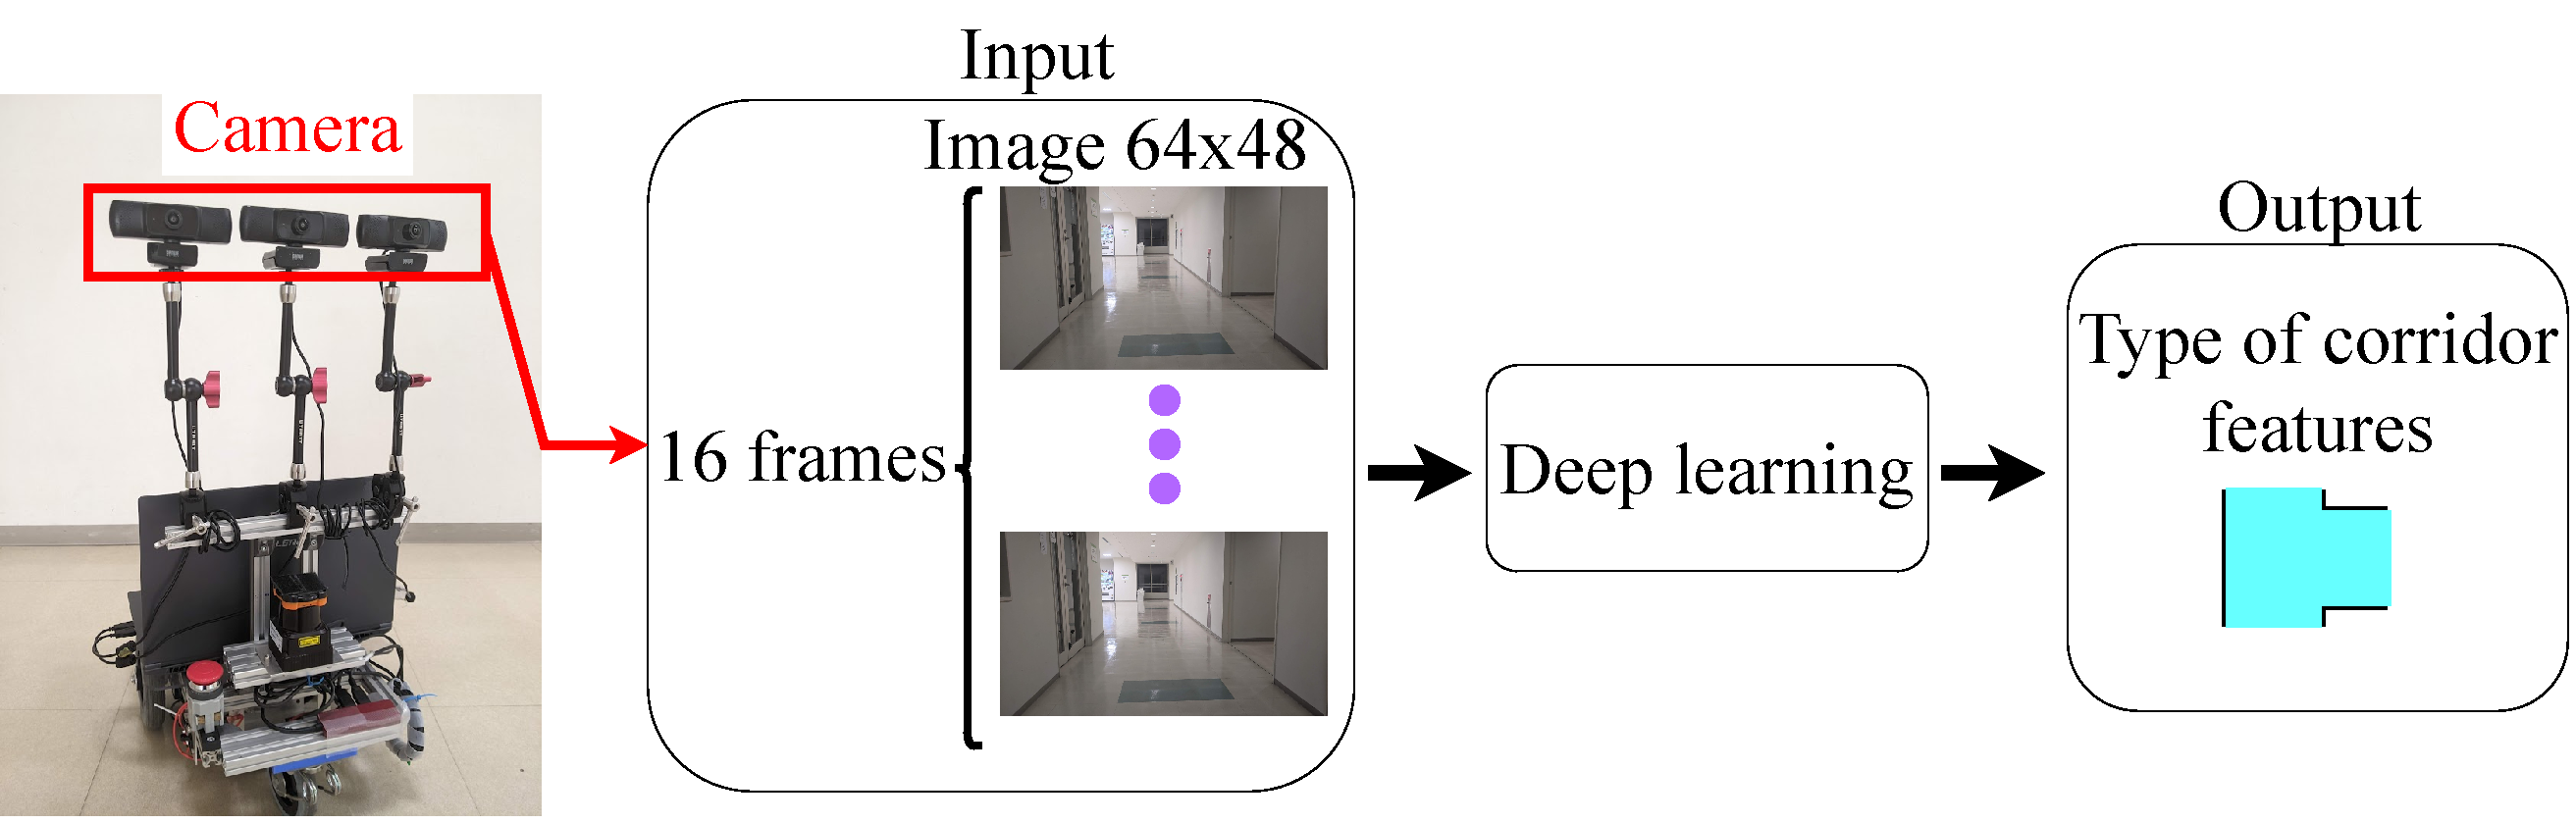
\includegraphics[height=28mm]{./figs/corridor_class.pdf}
     \caption{Overview of the corridor classification module}\label{fig:lrcn}
\end{figure}
\begin{figure}[h!]
    \centering
    %  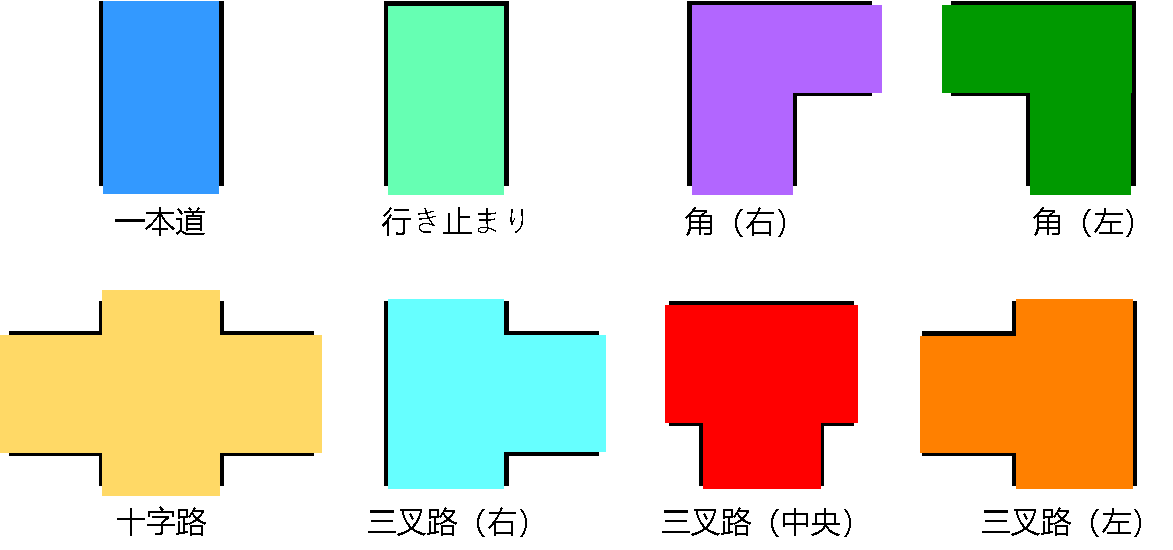
\includegraphics[height=40mm,width=80mm]{./figs/corridor.pdf}
     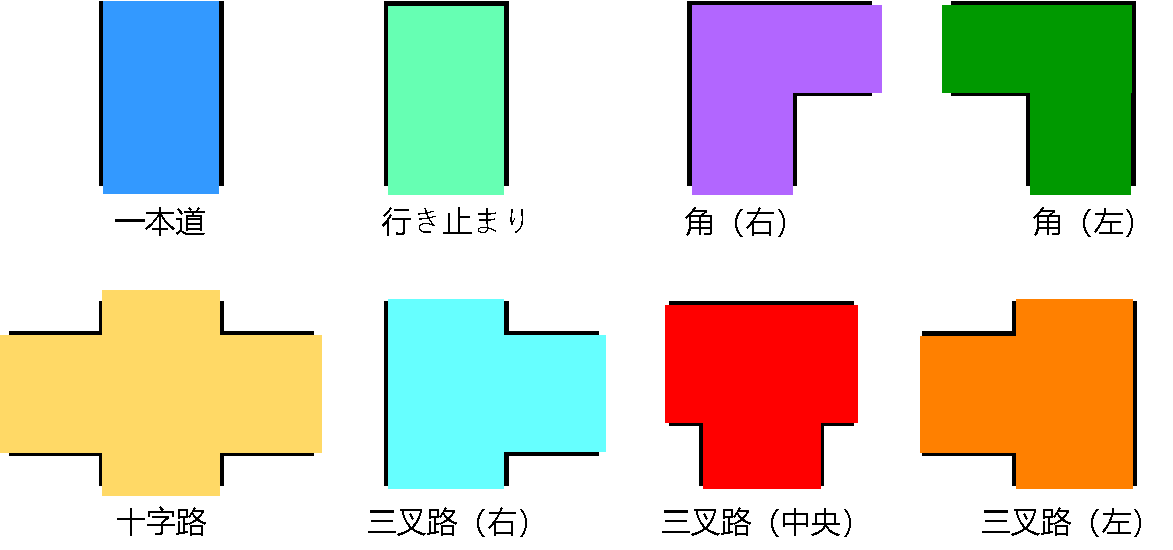
\includegraphics[height=36mm]{./figs/corridor.pdf}
     \caption{Types of corridor features}\label{fig:intersection}
\end{figure}
\par
次に通路分類モジュールのデータセットの作成について述べる.
データの作成では,経路追従モジュールの学習と同様に,
メトリックマップに基づいたルールベース制御器によって経路を走行する.
その際,フレーム数16の連続したカメラ画像と
通路の分類ラベルを1組とし,0.125秒周期でデータセットへ加える.
分類ラベルのアノテーションは,Fig.\ref{fig:map2label}に示すように,
通路の特徴を予め地図に登録しておくことで,自動的に行う.
% なお,分類ラベルのアノテーションは,Fig.\ref{fig:map2label}に示すように
% メトリックマップに基づいたルールベース制御器の出力を用いて,自動的に行う.
\begin{figure}[h!]
    \centering
    %  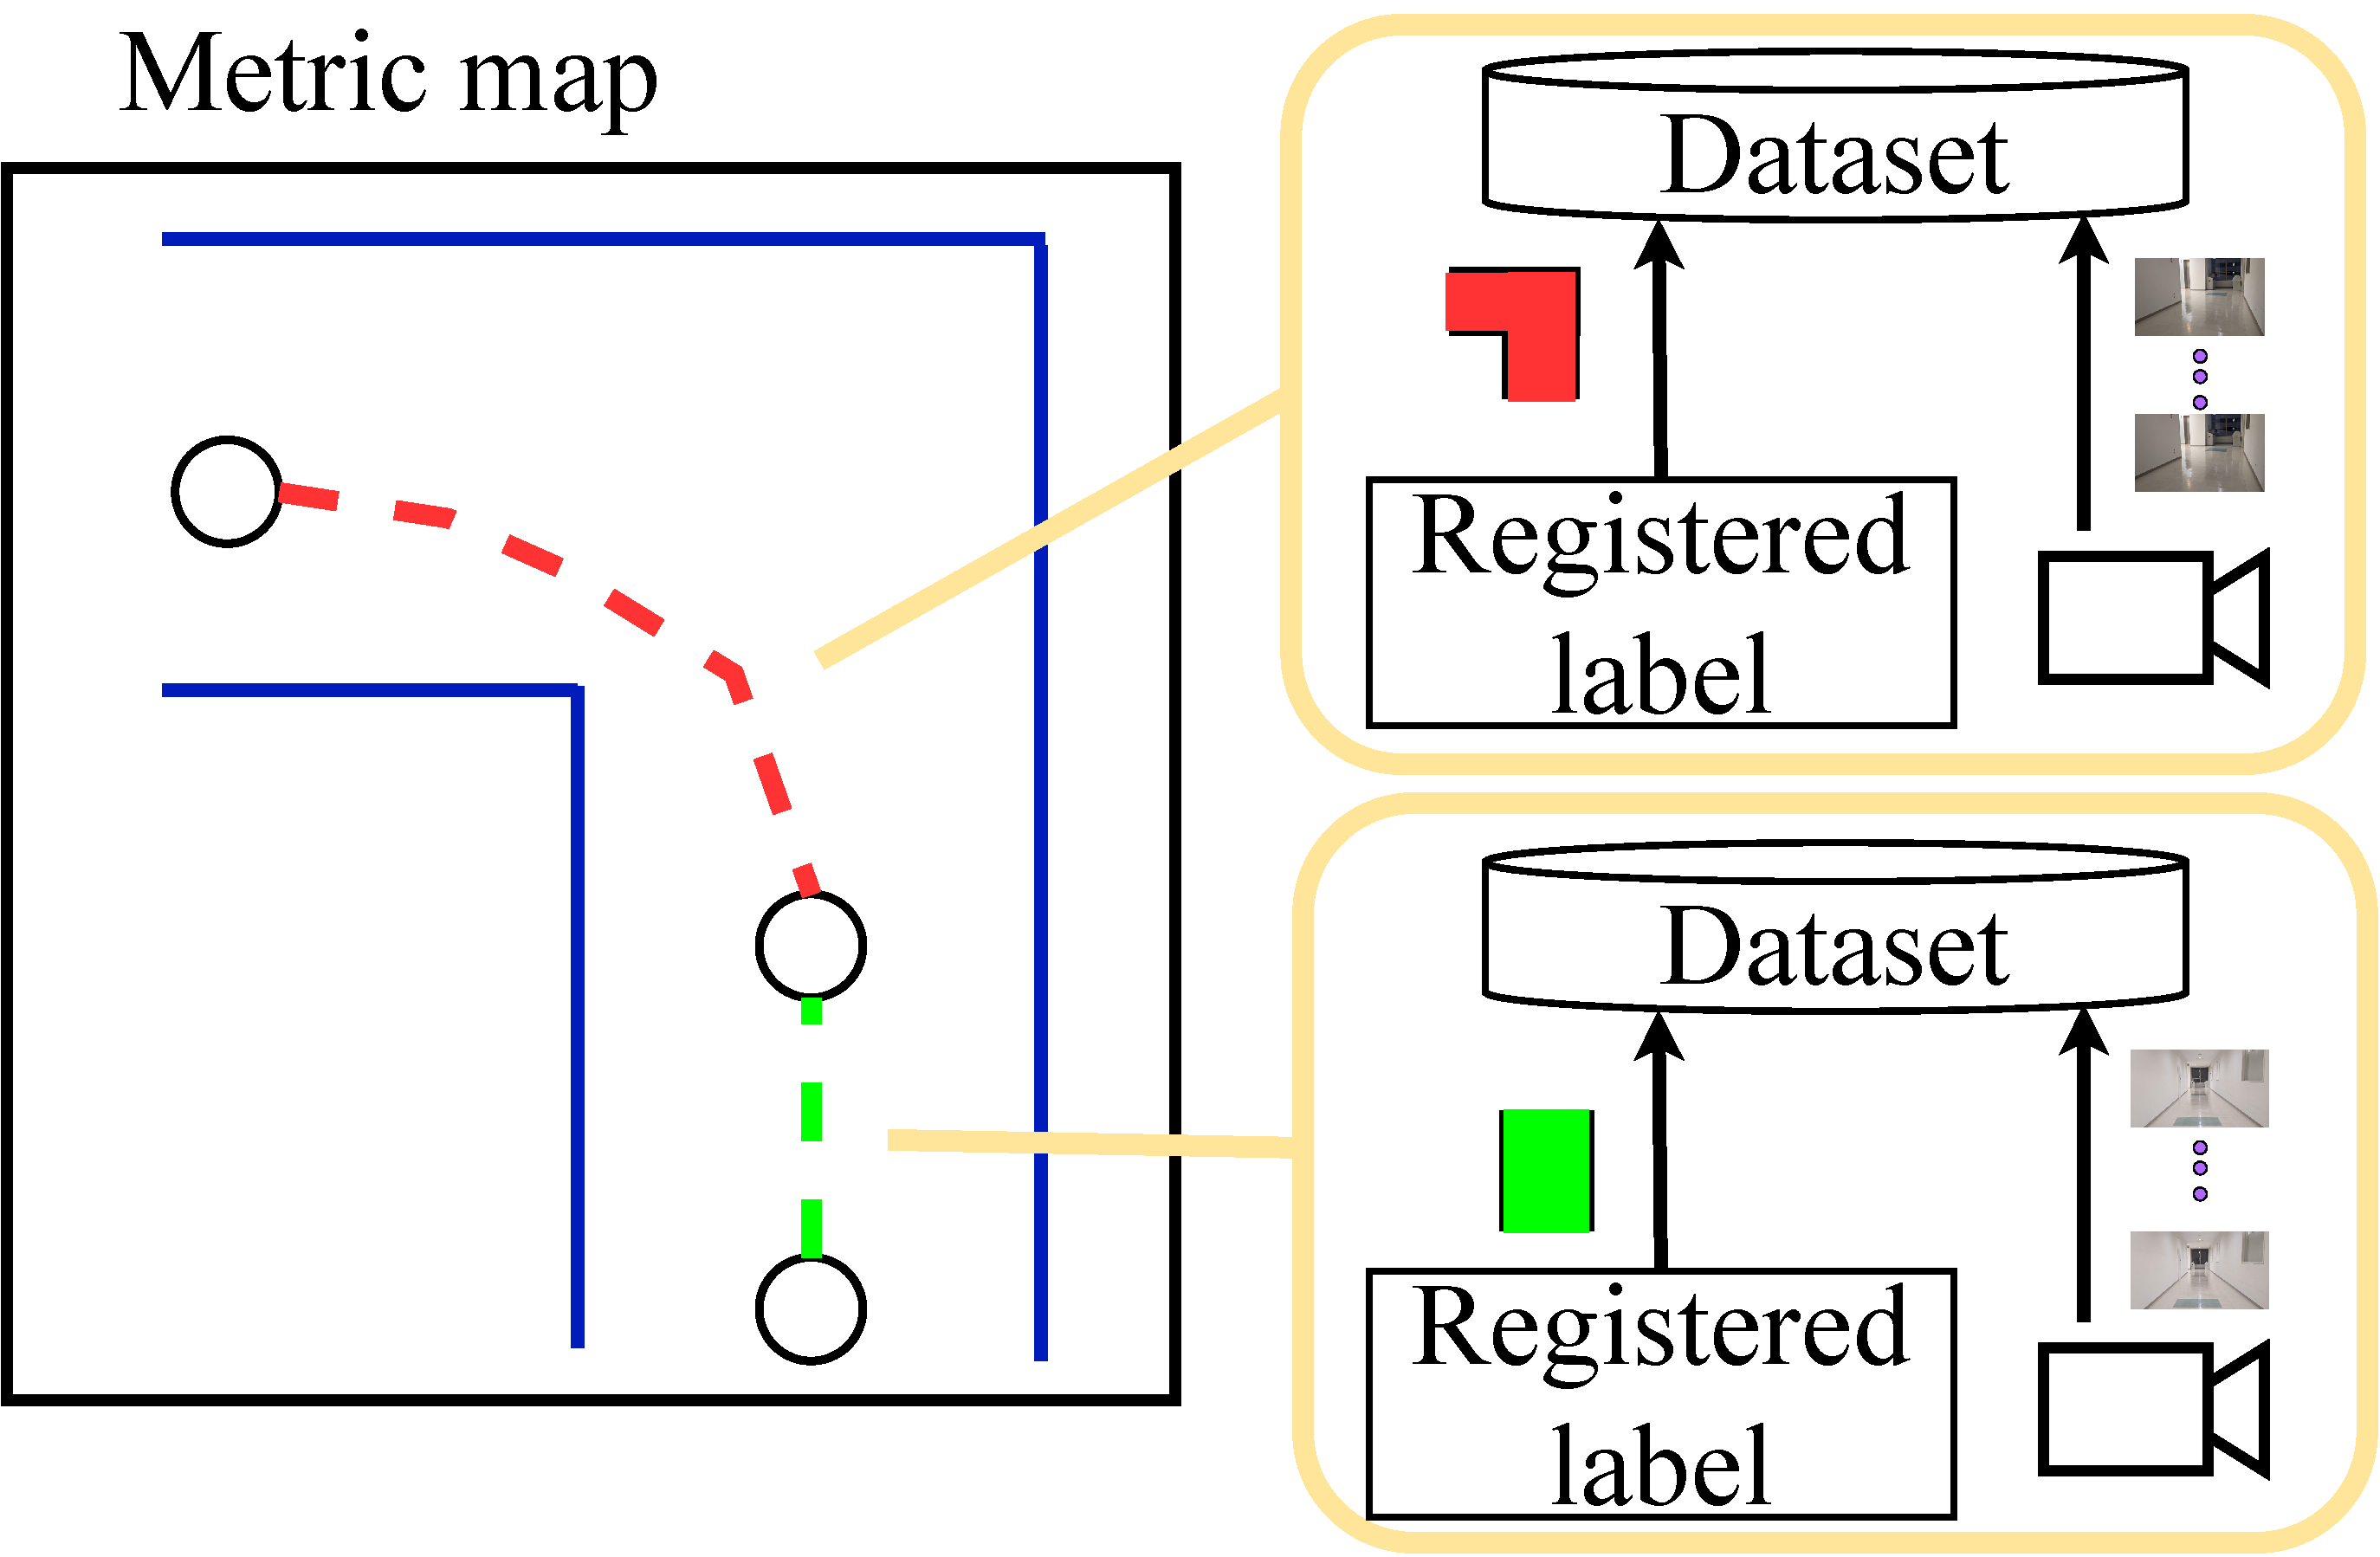
\includegraphics[height=40mm,width=80mm]{./figs/map_label.pdf}
     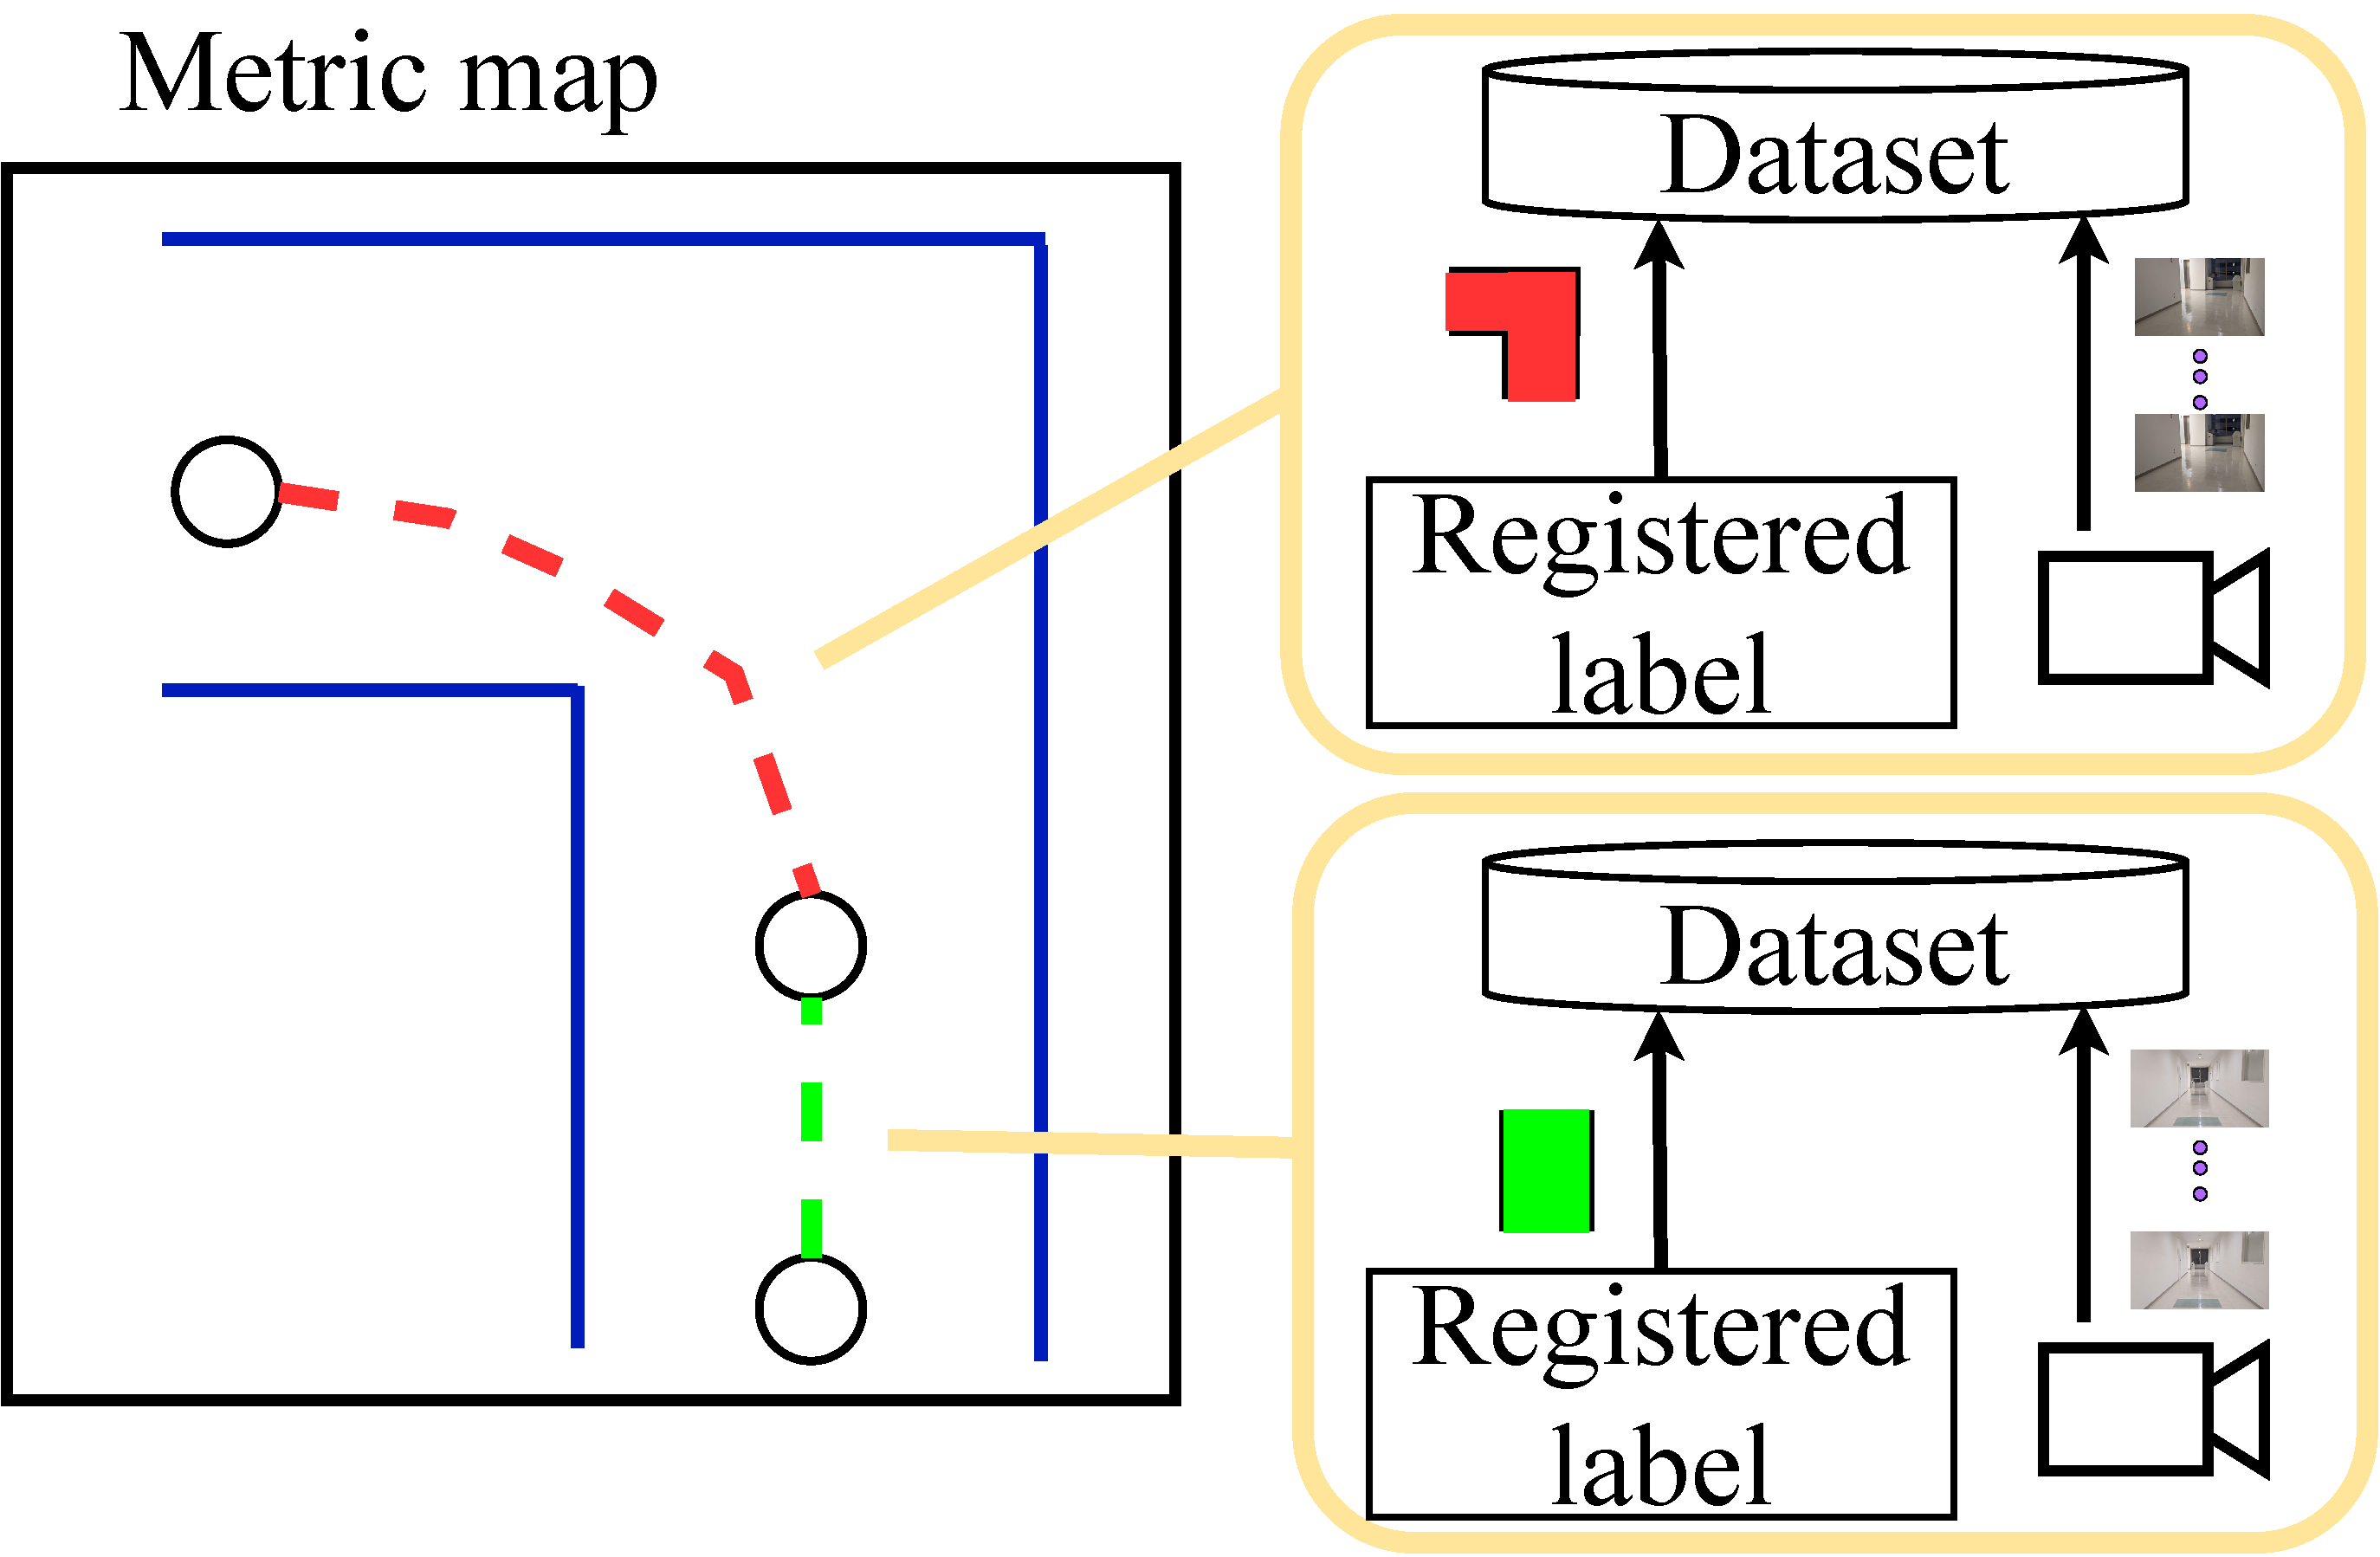
\includegraphics[height=38mm]{./figs/map_label.pdf}
     \caption{Classification labels registered in the metric map}\label{fig:map2label}
\end{figure}
\par
学習するデータセット内で,各クラスのデータ数が大きく異なる不均衡データは,
分類に大きな影響を与える
\cite{hukin}
とされている.
そのため,本稿では学習する際に,データセット内のクラス間のデータ数によって
重み付けを行うコストアプローチ\cite{cost}を導入している.

\section{実験}
実ロボットを用いて,提案するシステムにより,
ロボットが目的地へ到達可能であるか検証する.
% 提案するシステムによって,ロボットが目的地へ到達可能
% であるか,実ロボットを用いた実験により検証する.
\subsection{実験装置}
実験にはFig.\ref{fig:gamma}で示すロボットを使用する.
単眼ウェブカメラを3つ,2D-LiDAR(北陽電機 UTM-30LX)を1つ搭載して
いる.制御用のPCには(GALLERIA GCR2070RGF-QC-G)を使用している.
\begin{figure}[htbp]
    \centering
     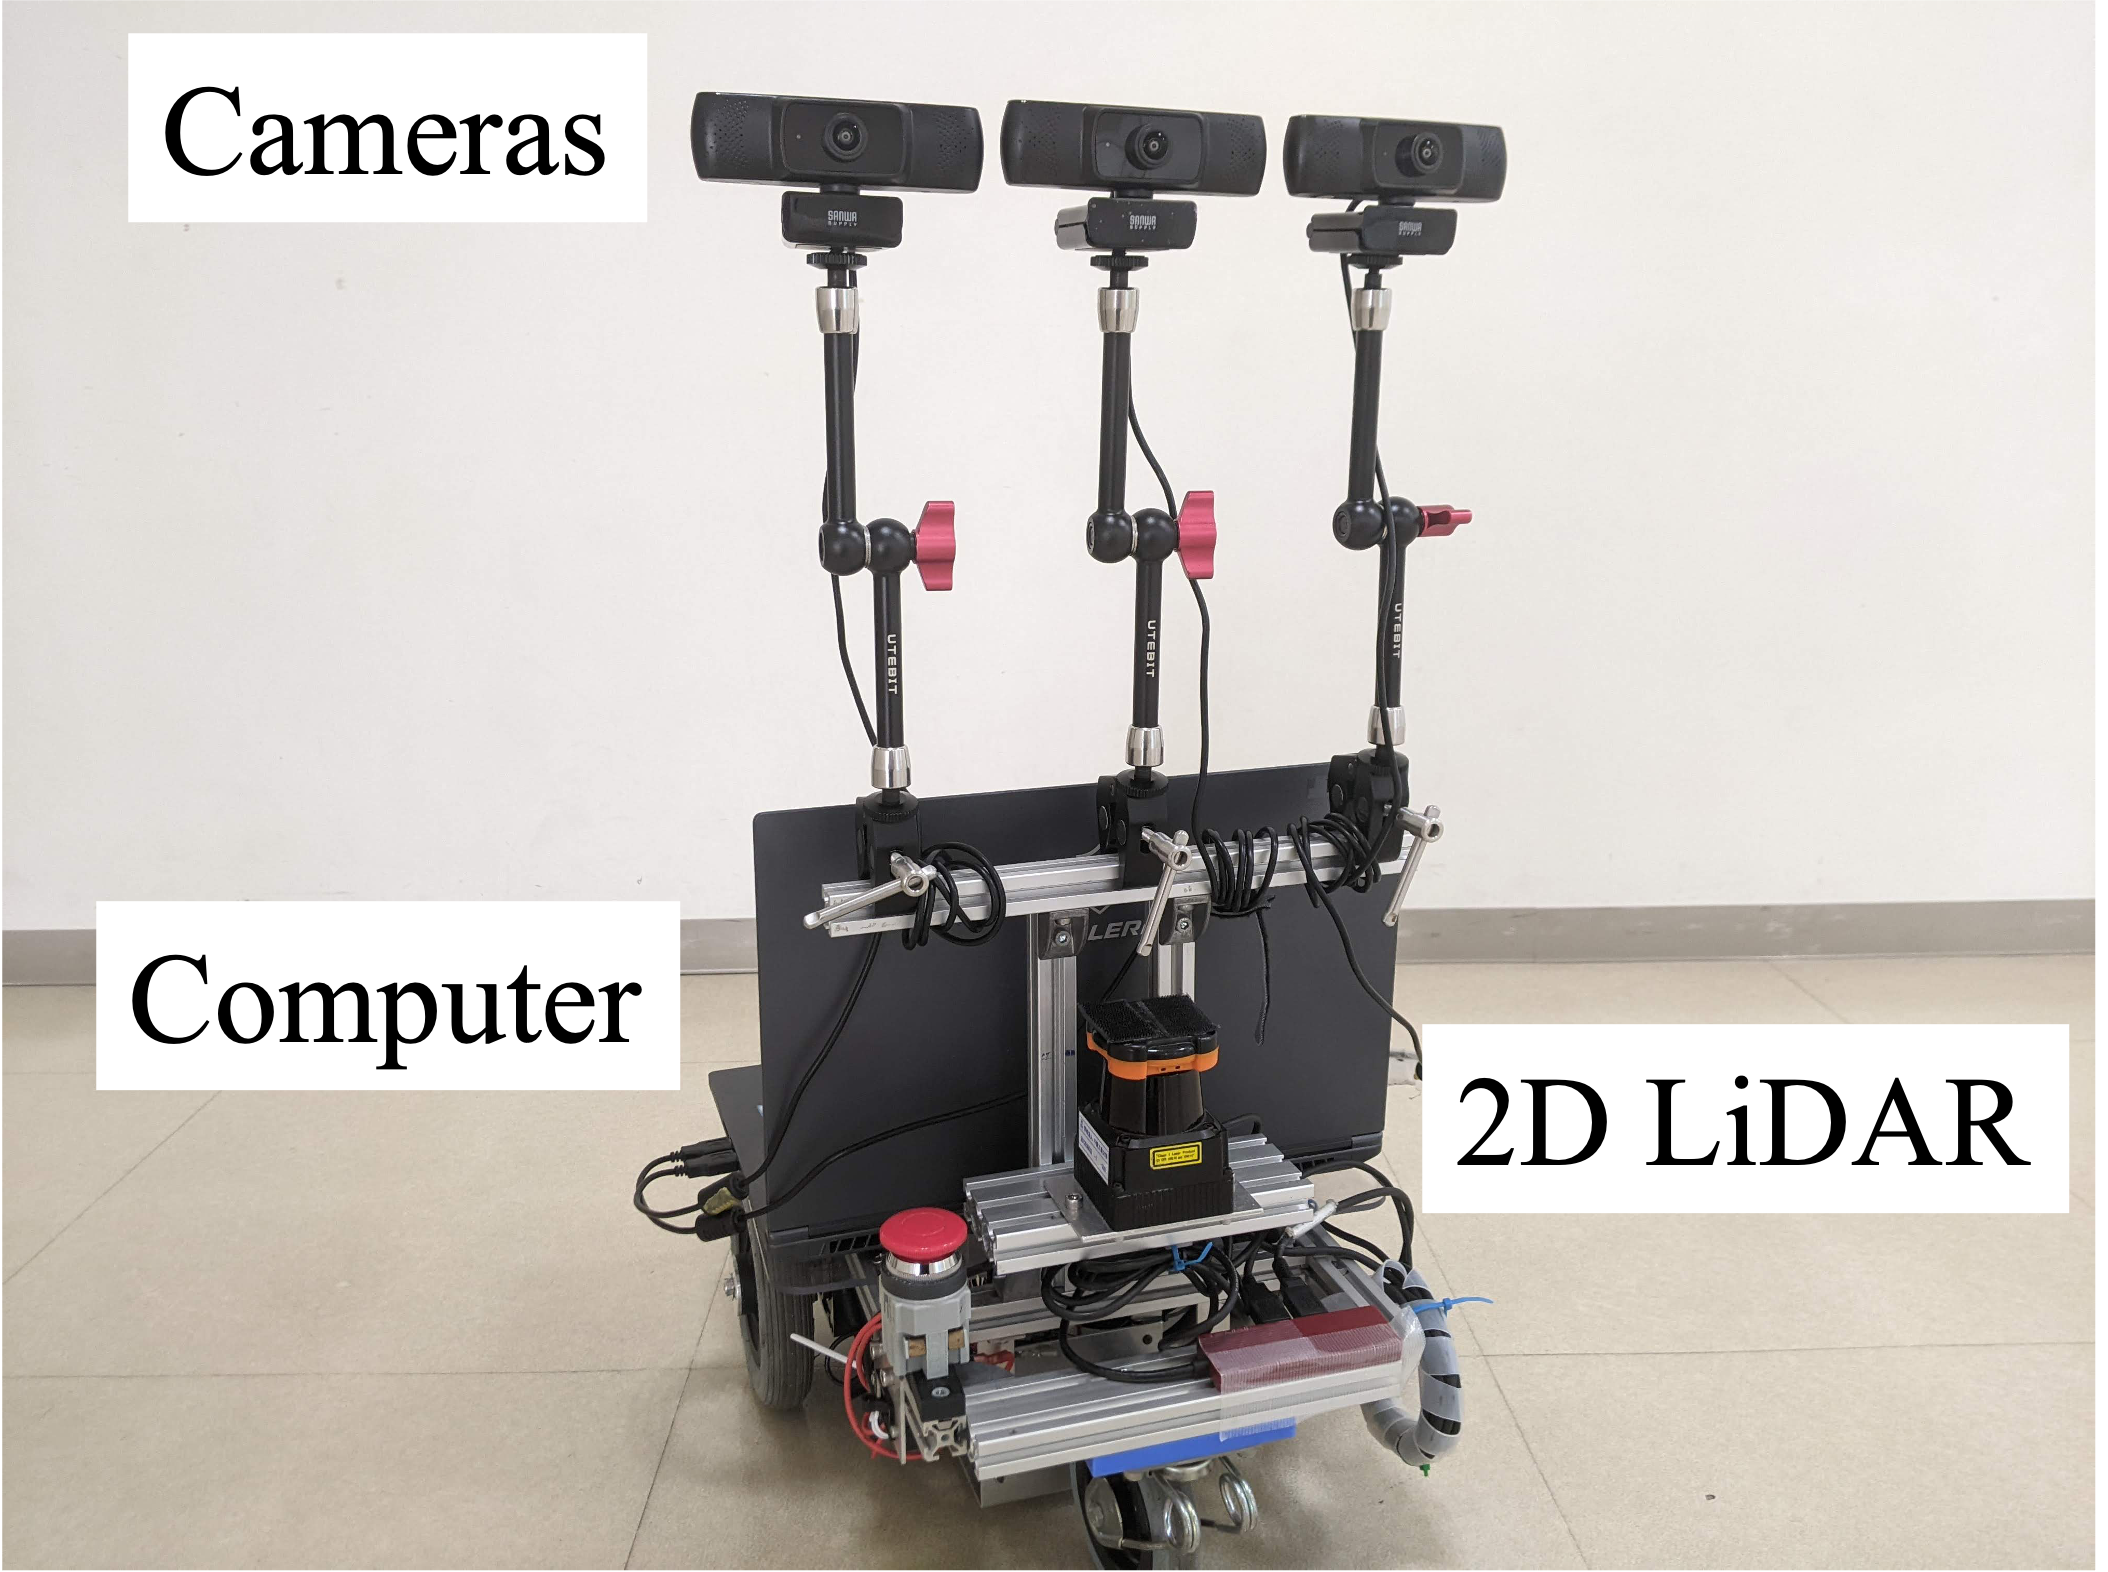
\includegraphics[height=38mm]{./figs/gamma_sensor.png}
     \caption{Experimental setup}\label{fig:gamma}
\end{figure}
\subsection{実験方法}
実験環境としてFig.\ref{fig:cit3f}に示す千葉工業大学津田沼キャンパス2号館3階の廊下を用いる.
% [藤原]と比較すると,突き当りが追加され,
% CとDが2つのこと行動を取ることが可能な分岐路へ変化している.
% 経路[藤原]で用いたa~fに図=で示したc~を追加した,a~nの順で走行する
% 前報と比較すると,突き当り,2つの行動がとれる分岐路C,Dが追加されている.
経路追従モジュールの訓練および通路分類モジュールのデータセット収集ではFig.\ref{fig:newroute}で示した
aからnの経路を順番に走行する.
実験では島田らが用いた50例のシナリオの中から,
Fig.\ref{fig:scenario_exp}に示す
7例を用いた.選定の基準は,Fig.\ref{fig:cit3f}の場所を対象としていること.
ロボットが移動困難な狭い通路が含まれていないこと.
「後ろを向く」など経路追従モジュールができない行動が含まれていないことである.
% Fig.\ref{fig:scenario_exp}に実験で用いた7例のシナリオを示す.
% Fig.\ref{fig:cit3f}に示したエリアを対象として抽出した7例を用いる.
% シナリオの抽出において,1.メトリックマップを用いたルールベース制御器で通行が困難な場所が含まれるもの.
% 2.その場で「右を向く」といった経路追従モジュールが達成困難なもの
% を除外している.
% \par
まずはじめに通路分類モジュールの訓練を行う.
前述の経路をメトリックマップに基づいたルールベース制御器の出力を用いて,3周し,
データセットを収集する.
収集したデータは,1,2周目を訓練データとし,3周目をテストデータとする.
それぞれのデータ数は,
訓練データ5781,テストデータ2902である.
訓練はバッチサイズを32として,30epoch行った.
訓練の結果,テストデータに対するAccuracyは0.98であった.
次に経路追従モジュールの訓練を行う.
通路分類モジュールの訓練と同様の経路を,オンラインで模倣学習しながら1周走行する.
その際のステップ数は12000であった.
\par
2つのモジュールを訓練後,シナリオを1例ずつ入力して,ロボットの挙動を観察する.
実験では,ロボットをシナリオのスタート地点に移動して,自律移動を開始する.
\begin{figure}[htbp]
    \centering
    %  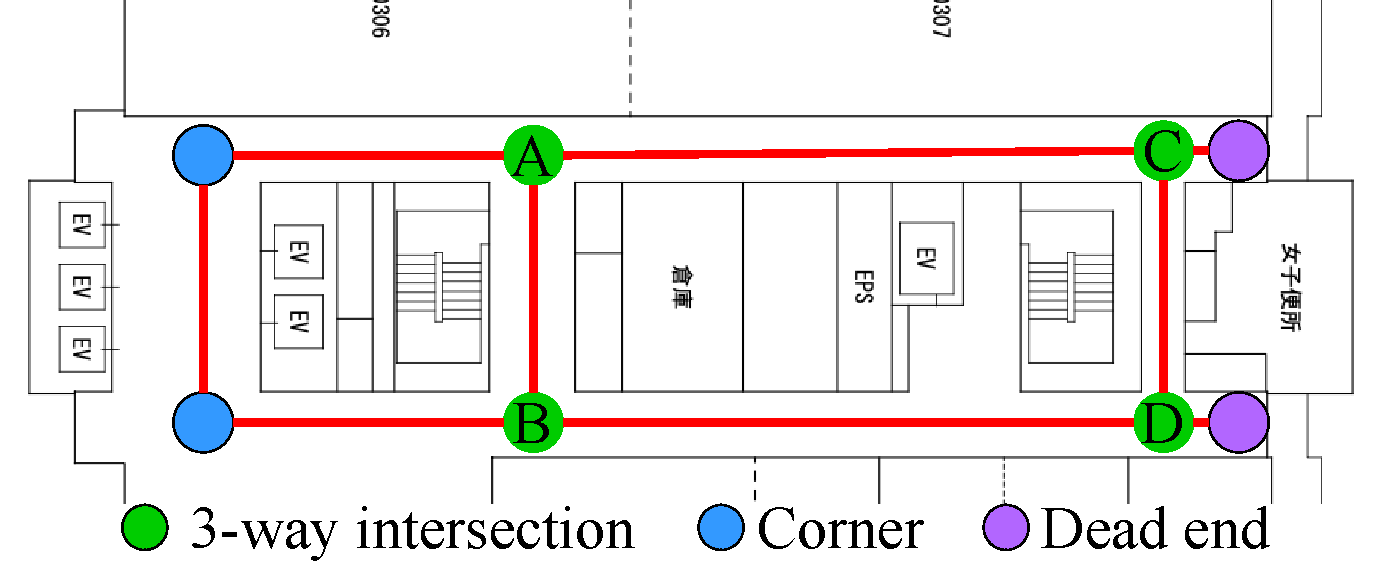
\includegraphics[height=40mm,width=80mm]{./figs/cit3f.pdf}
     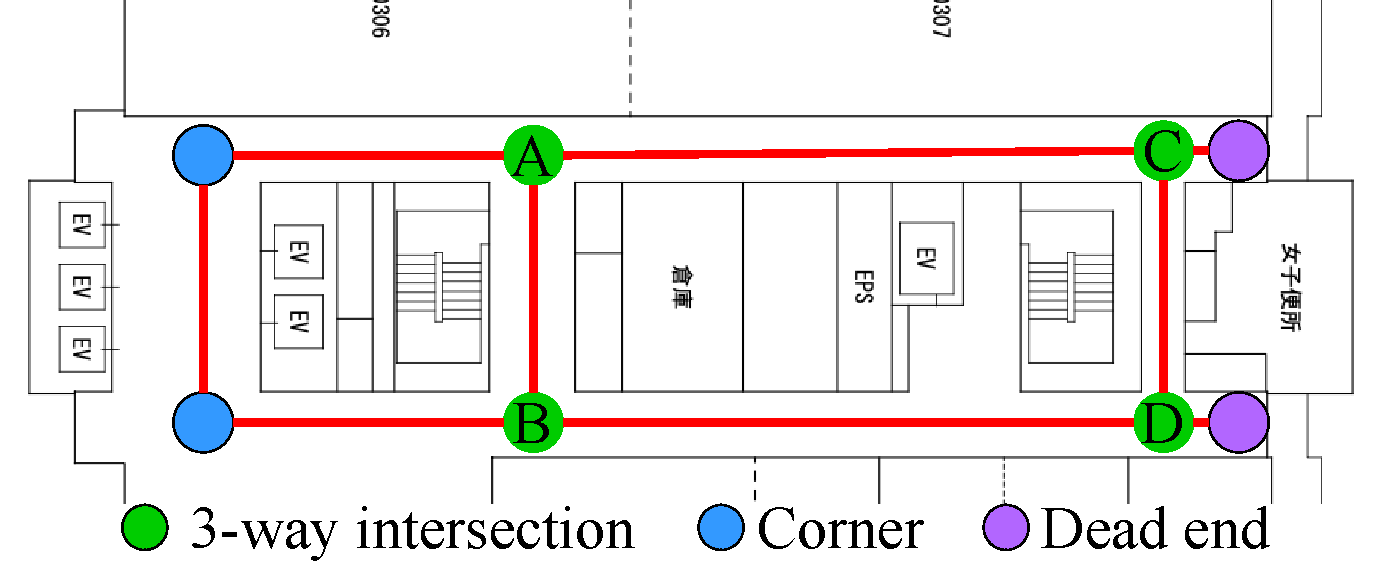
\includegraphics[height=38mm]{./figs/cit3f.pdf}
     \caption{Experimental environment}\label{fig:cit3f}
\end{figure}

\subsection{実験結果}
Fig.\ref{fig:exp_path}にFig.\ref{fig:scenario24}のシナリオを入力した実験の様子
を示す.図に示すように,シナリオの道順に従い,
三叉路などの分岐路で適切に経路を選択して
自律移動する様子が見られた.結果として,7例すべ
てでロボットが,目的地へ到達した.
以上の結果から,提案するカメラ画像
とシナリオに基づいて,経路を追従して目的地まで自
律移動するシステムの有効性が確認された.
% 7例すべての例でロボットは指定された経路を追従して目的地へ到達した.
% % 実験結果をTable \ref{tab:result}に示す.
% % 表はそれぞれ実験に用いたシナリオの番号,学習器の出力が要因による介入の回数,
% % 通路分類の間違いを要因とする介入の回数である.
% Fig.\ref{fig:exp_path}にFig.\ref{fig:scenario24}のシナリオを入力した実験の様子を示す.
% 図に示すように,シナリオで指定された道順に従い,三叉路などの分岐路で
% 適切に経路を選択して目的地まで自律移動する様子が見られた.
% 結果として,7例すべての例でロボットは指定された経路を追従して目的地へ到達した.
% 以上の結果から,提案するカメラ画像とシナリオに基づいて,
% 経路を追従して目的地まで自律移動するシステムの有効性が確認された.
% シナリオに基づくナビゲーションとカメラ画像による通路分類を追加したシステムが,
% 適切に動作することを確認した.
\section{結言}
本稿では,事前に作成したメトリックマップを用い
ず,カメラ画像とシナリオに基づいて経路を追従して
目的地まで自律移動するシステムを提案した.そして,実
ロボットを用いた実験により提案システムの有効性を検証
した.実験では,提案システムにより,ロボットが目的地
へ到達可能であることを確認した.
\printbibliography[title=参考文献]
\begin{figure*}[htbp]
    \centering
    %  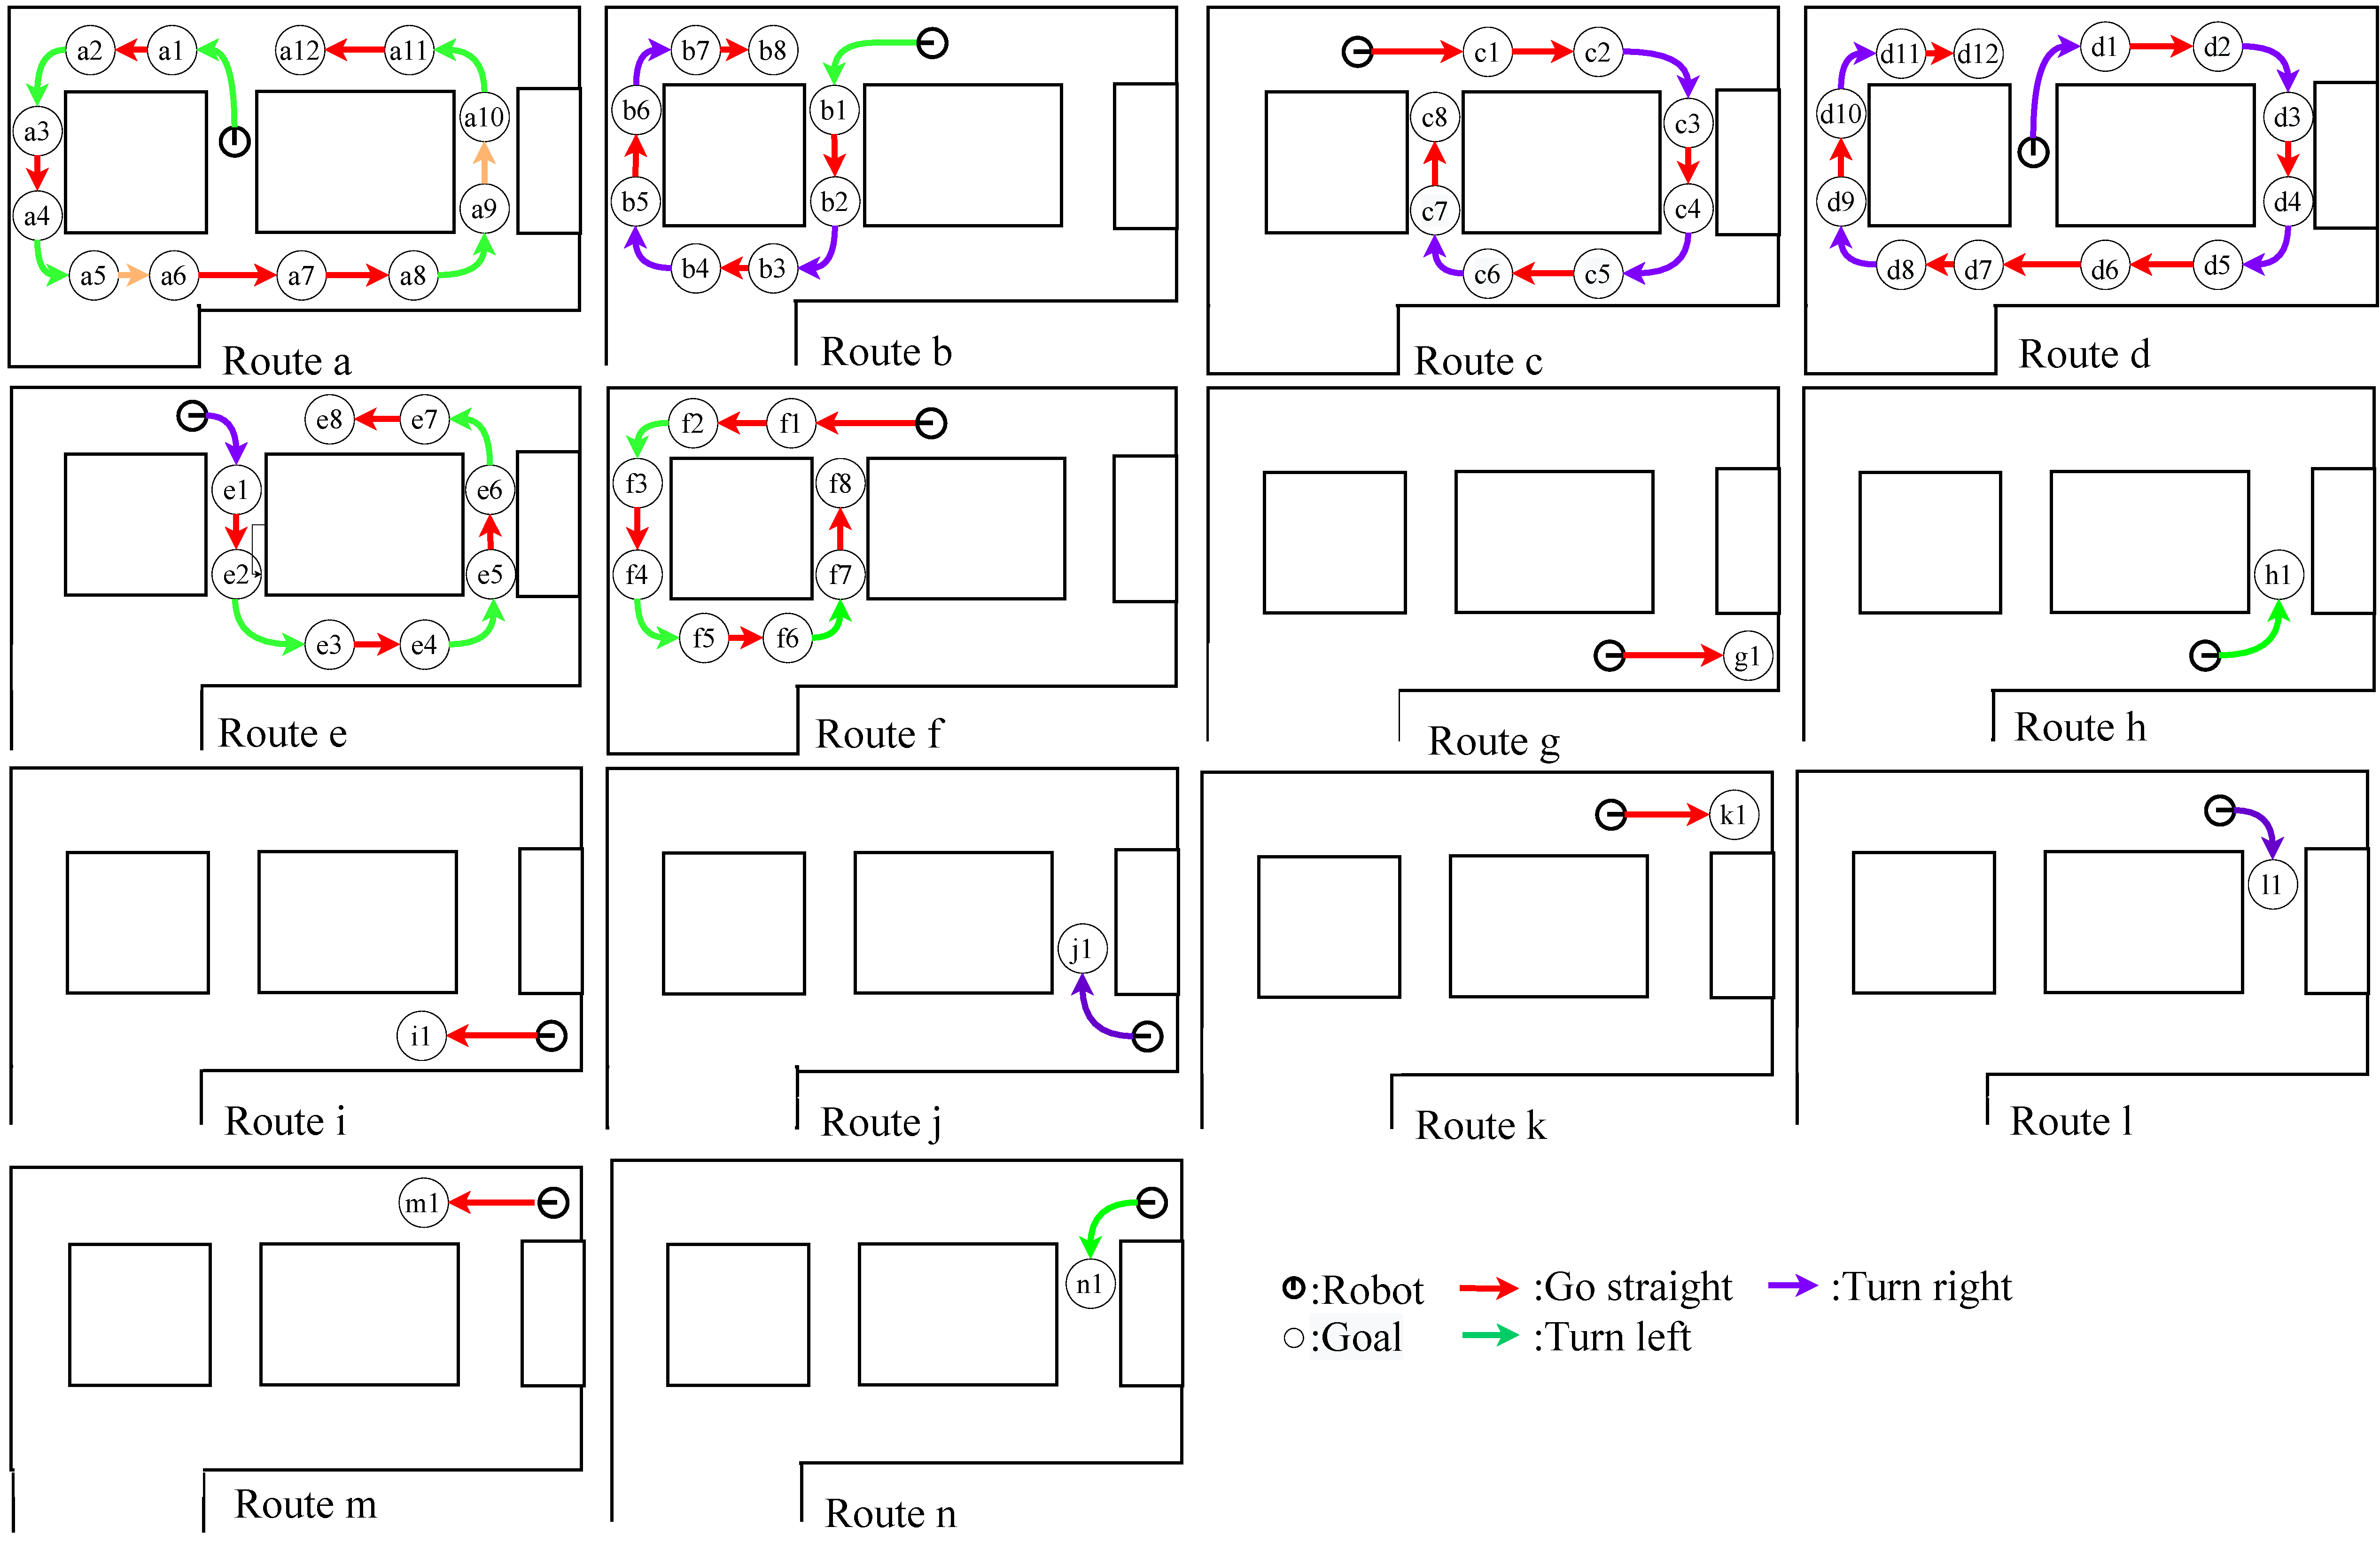
\includegraphics[height=120mm,width=160mm]{./figs/newroute.pdf}
     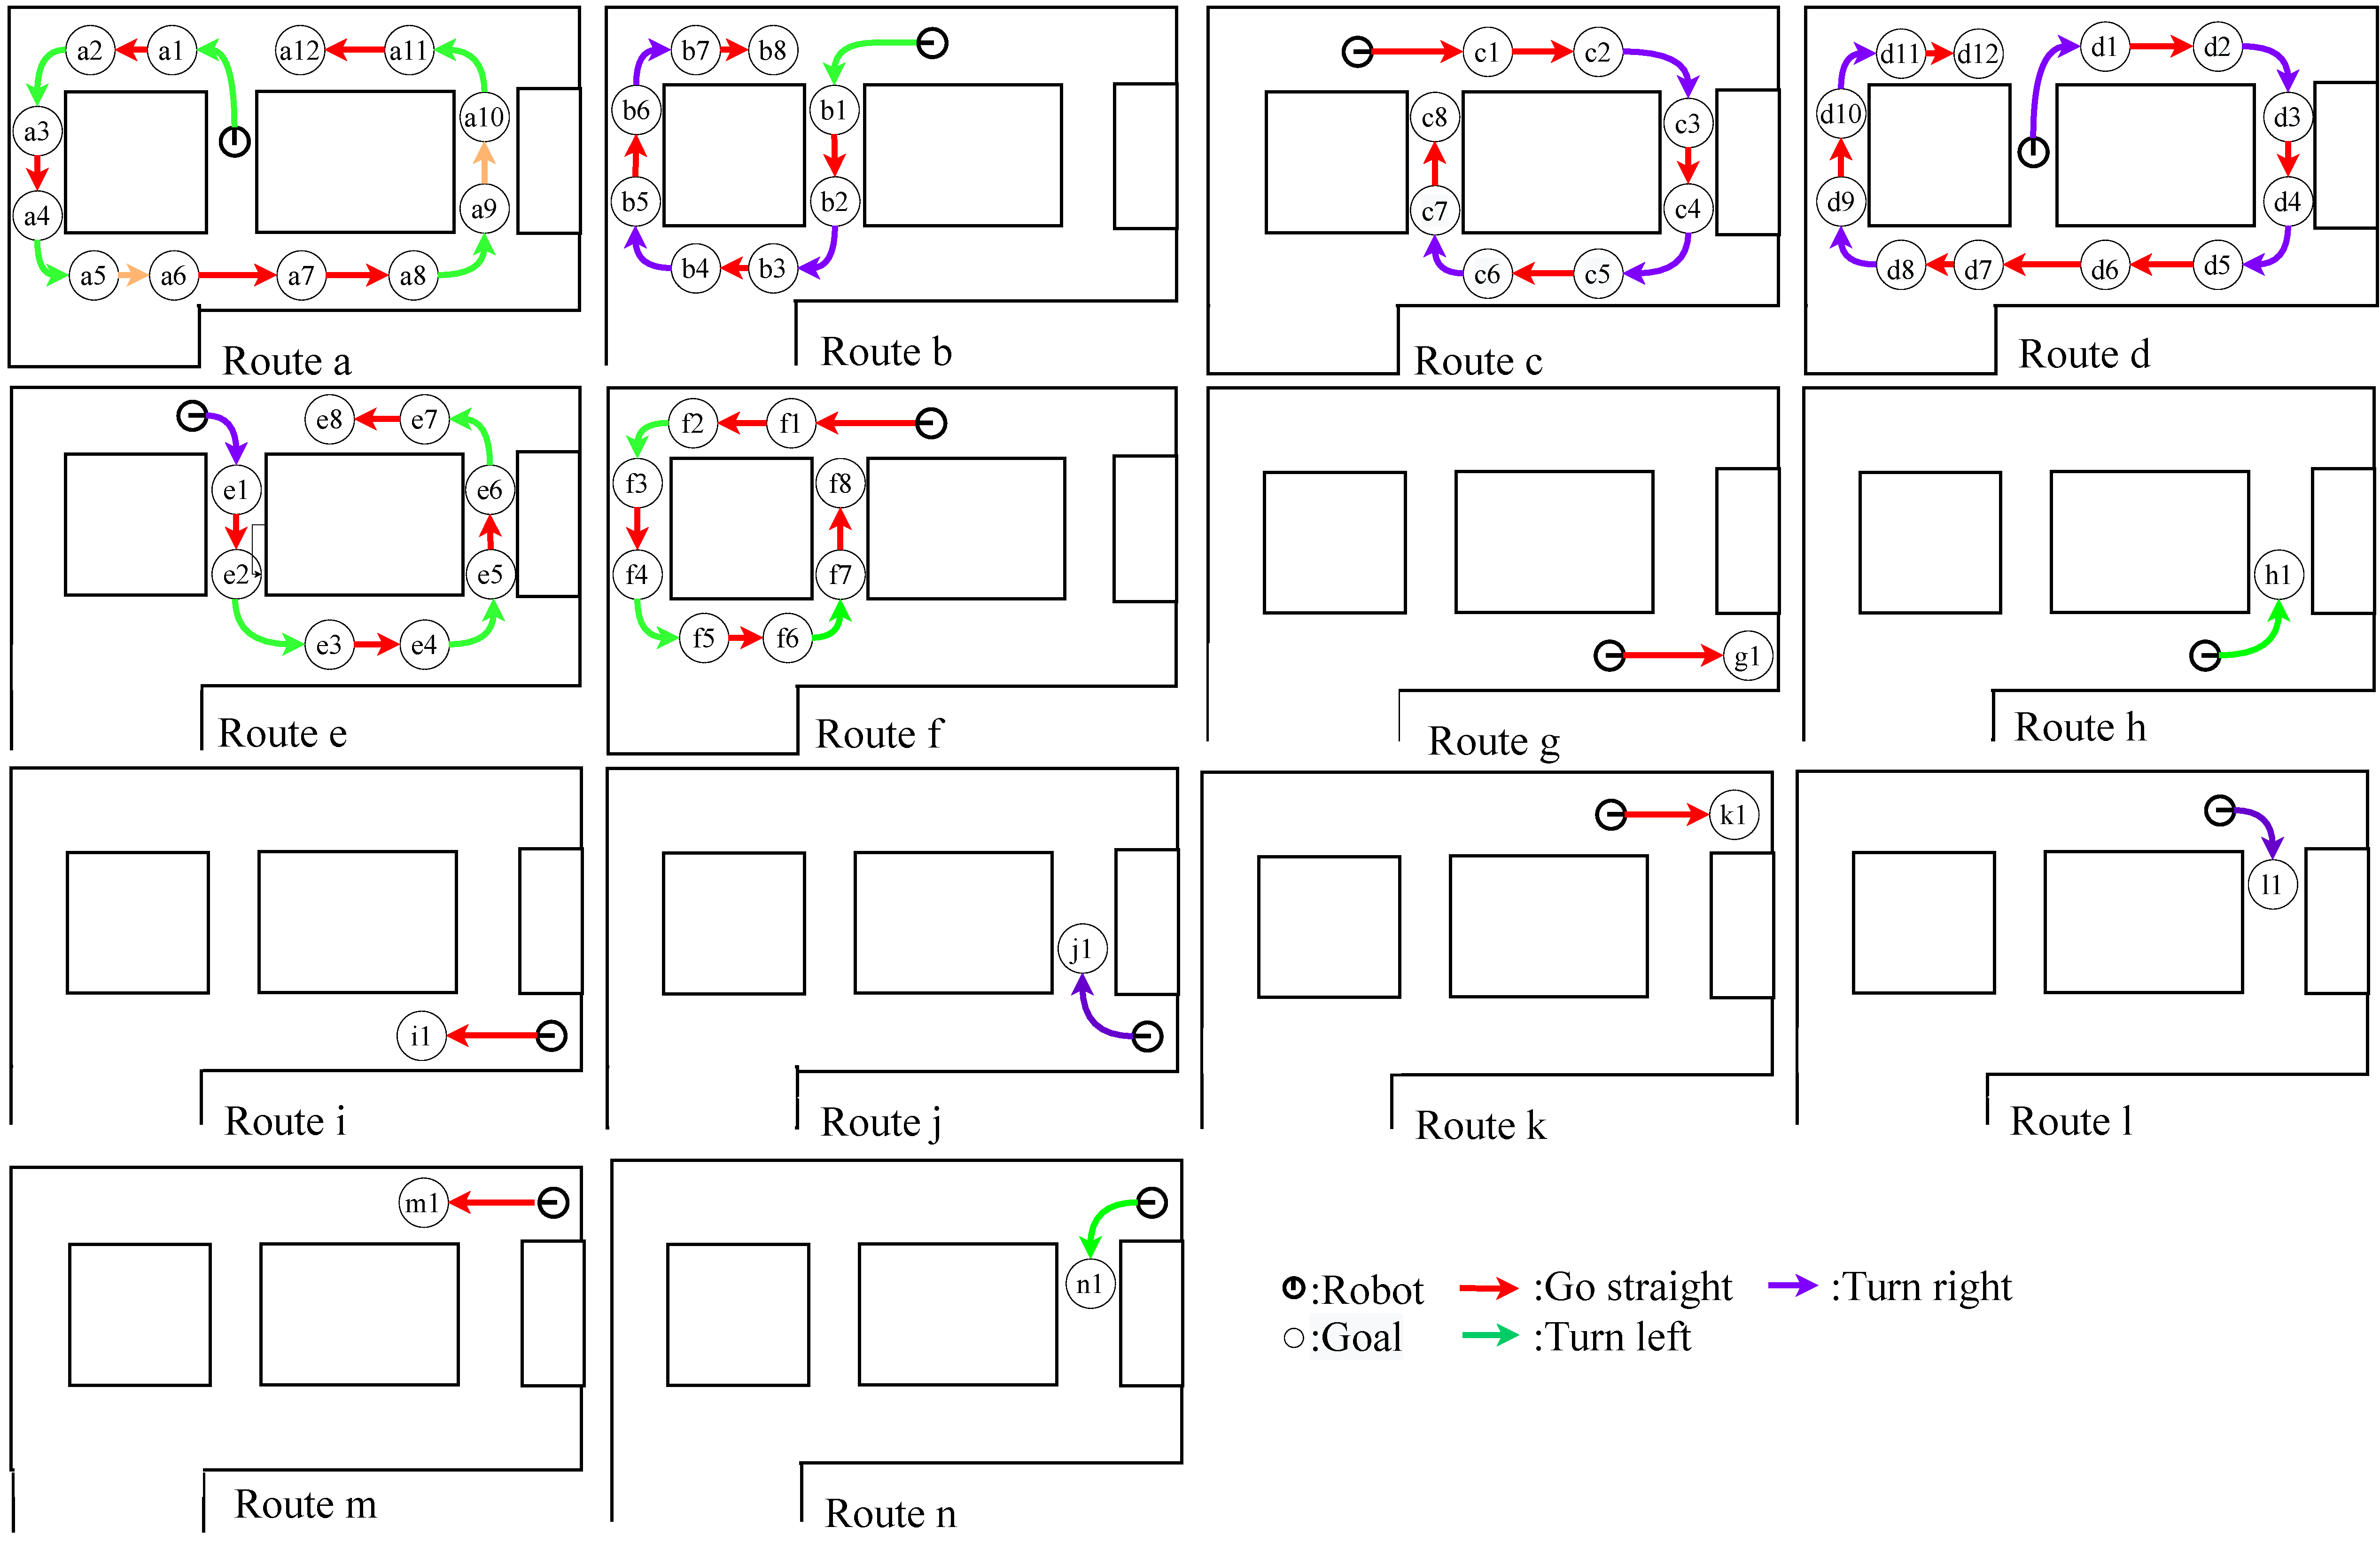
\includegraphics[height=120mm]{./figs/newroute.pdf}
     \caption{Route used for learning}\label{fig:newroute}
\end{figure*}
\begin{figure*}[htbp]
    \begin{tabular}{ccc}
        \begin{minipage}[t]{0.3\textwidth}
            \centering
            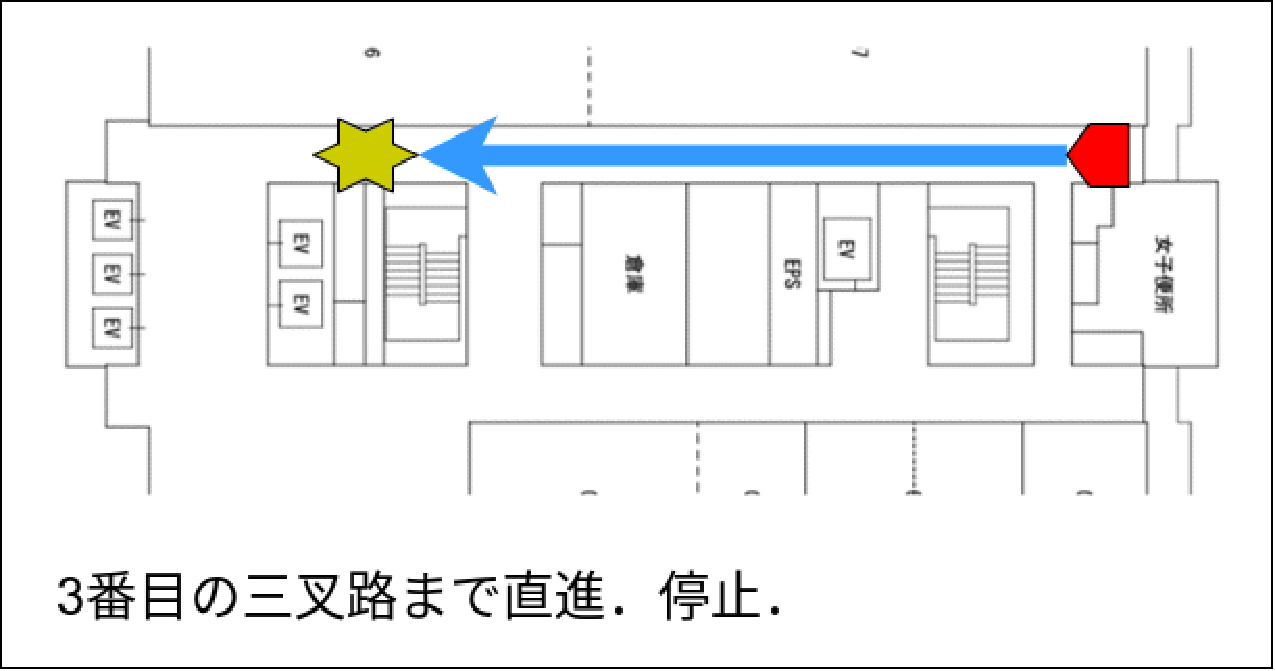
\includegraphics[keepaspectratio, width=57mm]{figs/scenario/scenario01.pdf}
            \subcaption{Scenario 01}
            \label{composite}
        \end{minipage} &
        \begin{minipage}[t]{0.3\textwidth}
            \centering
            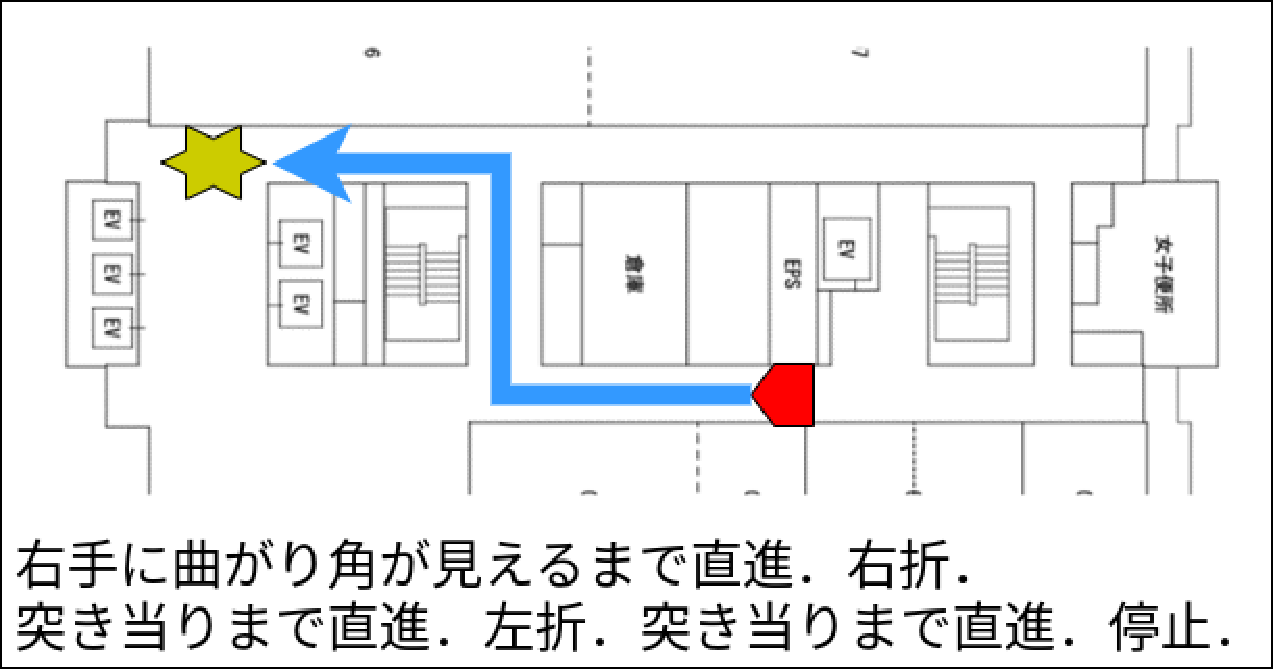
\includegraphics[keepaspectratio, width=57mm]{figs/scenario/scenario02.pdf}
            \subcaption{Scenario 02}
            \label{Gradation}
        \end{minipage} &
        \begin{minipage}[t]{0.3\textwidth}
            \centering
            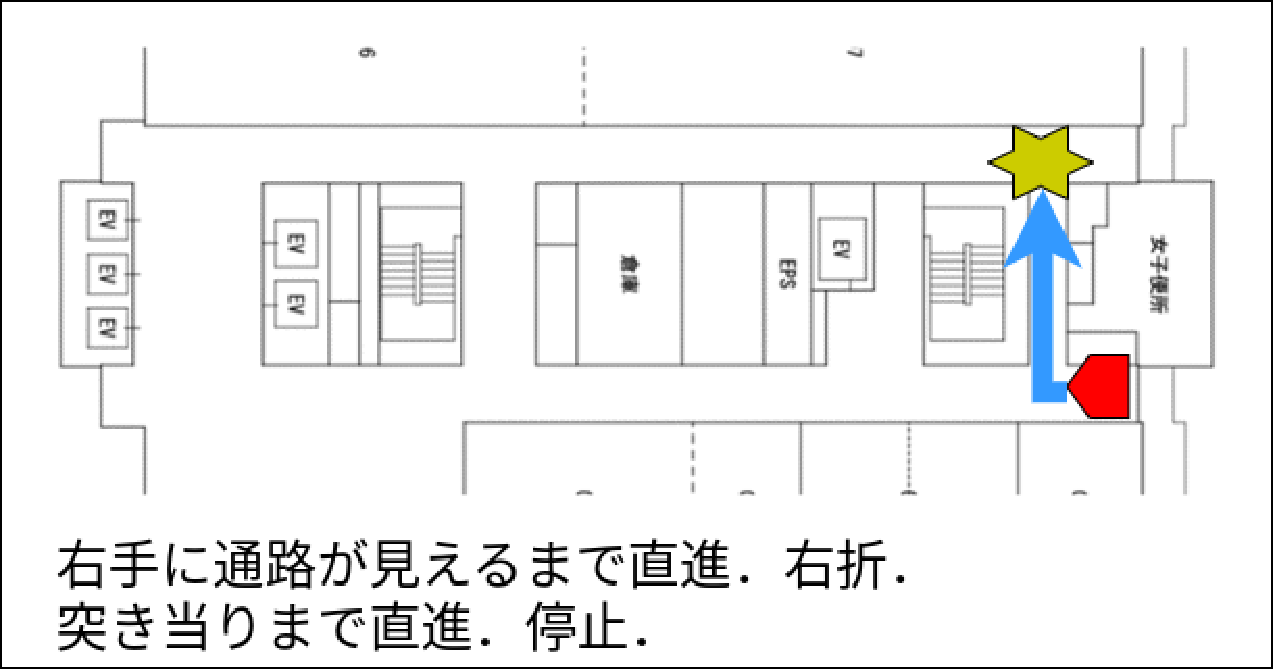
\includegraphics[keepaspectratio, width=57mm]{figs/scenario/scenario03.pdf}
            \subcaption{Scenario 03}
            \label{fill}
        \end{minipage} \\
        \begin{minipage}[t]{0.3\textwidth}
            \centering
            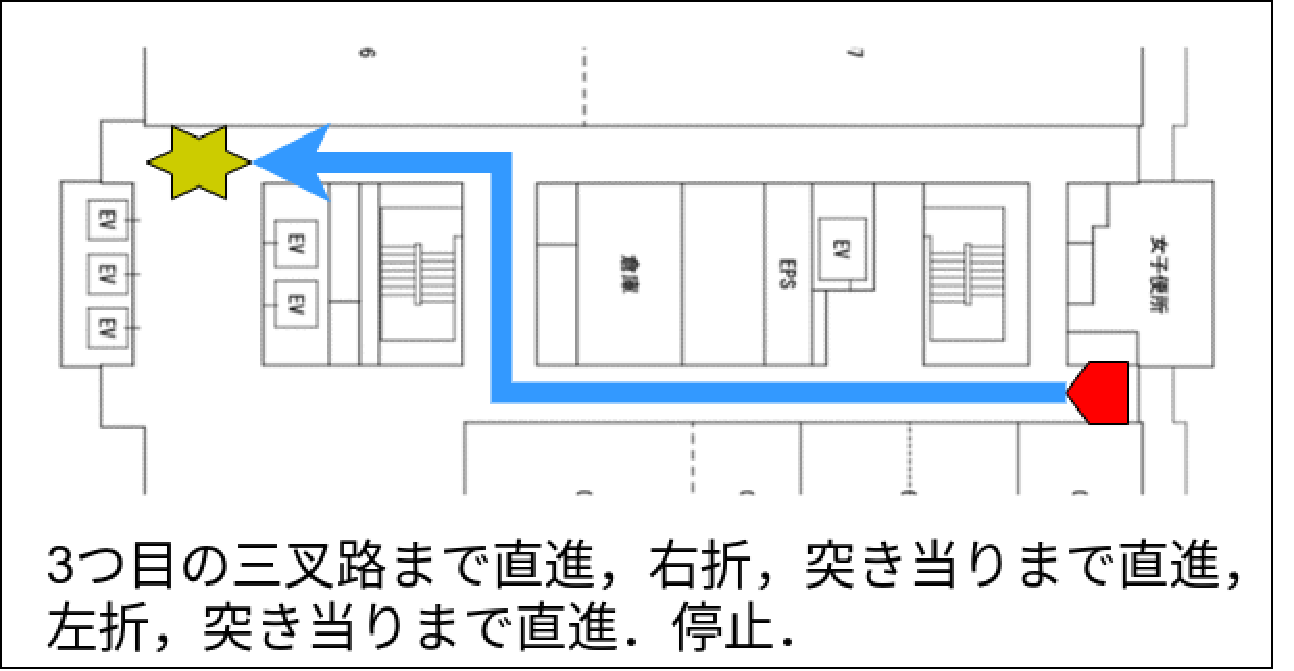
\includegraphics[keepaspectratio, width=57mm]{figs/scenario/scenario04.pdf}
            \subcaption{Scenario 04}
            \label{transform}
        \end{minipage} &
        \begin{minipage}[t]{0.3\textwidth}
            \centering
            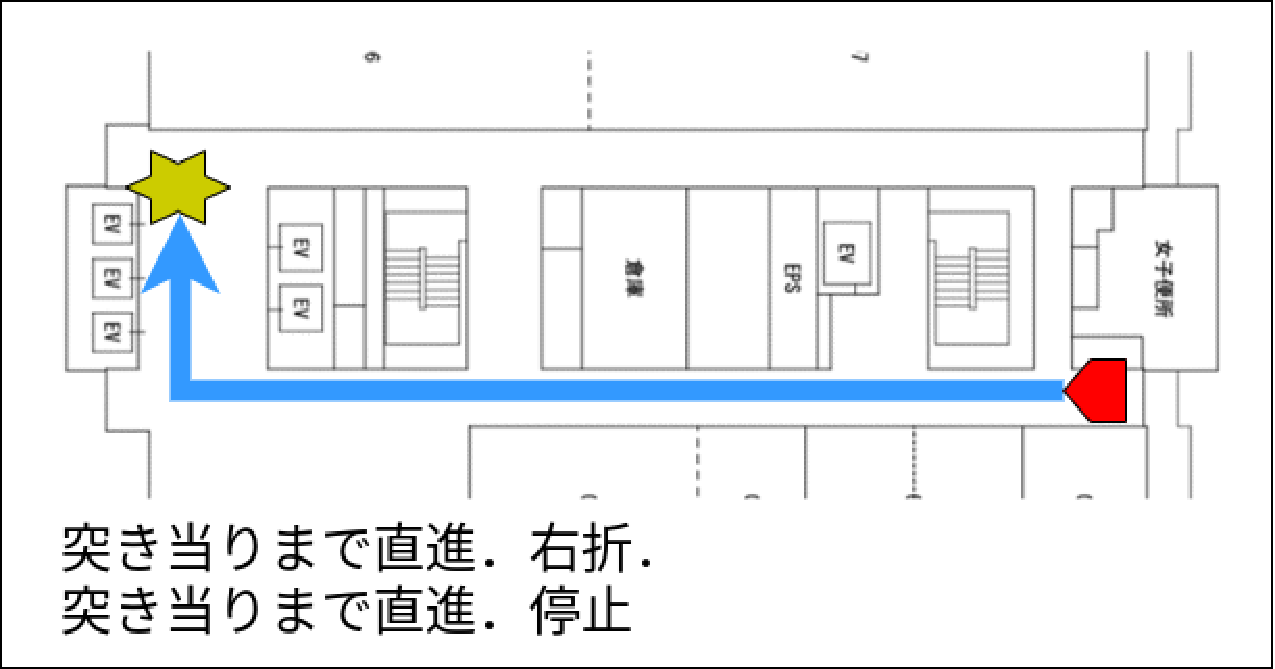
\includegraphics[keepaspectratio, width=57mm]{figs/scenario/scenario05.pdf}
            \subcaption{Scenario 05}
            \label{image1}
        \end{minipage} &
        \begin{minipage}[t]{0.3\textwidth}
            \centering
            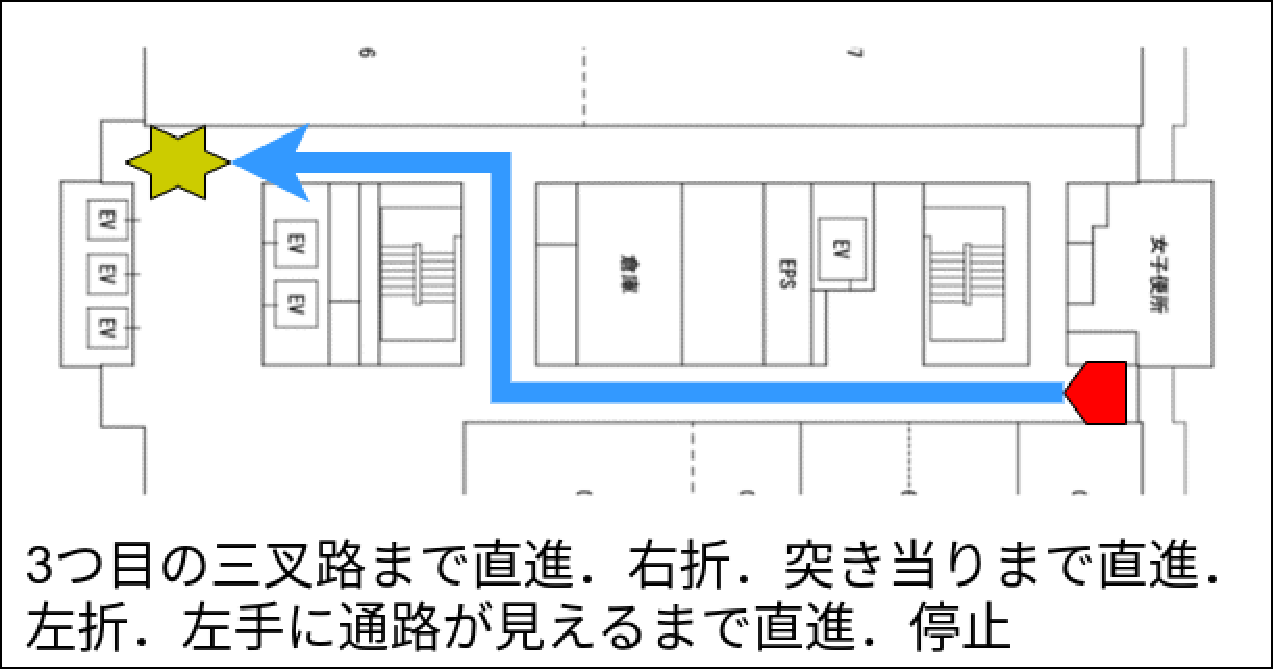
\includegraphics[keepaspectratio, width=57mm]{figs/scenario/scenario06.pdf}
            \subcaption{Scenario 06}
            \label{fig:scenario24}
        \end{minipage}\\
        \begin{minipage}[t]{0.3\textwidth}
            \centering
            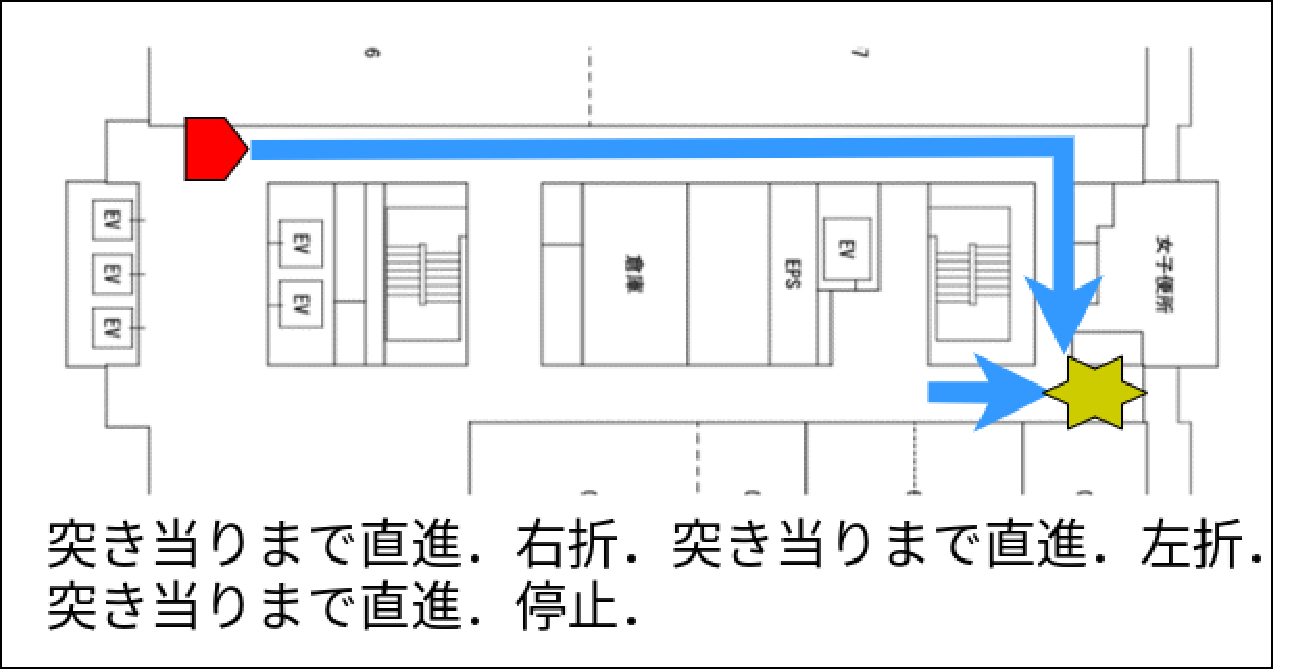
\includegraphics[keepaspectratio, width=57mm]{figs/scenario/scenario07.pdf}
            \subcaption{Scenario 07}
            \label{imagess}
        \end{minipage}
    \end{tabular}
    \caption{Scenarios used in the experiment}\label{fig:scenario_exp}
\end{figure*}

\begin{figure*}[htbp]
    \begin{tabular}{ccc}
        \begin{minipage}[t]{0.5\textwidth}
            \centering
            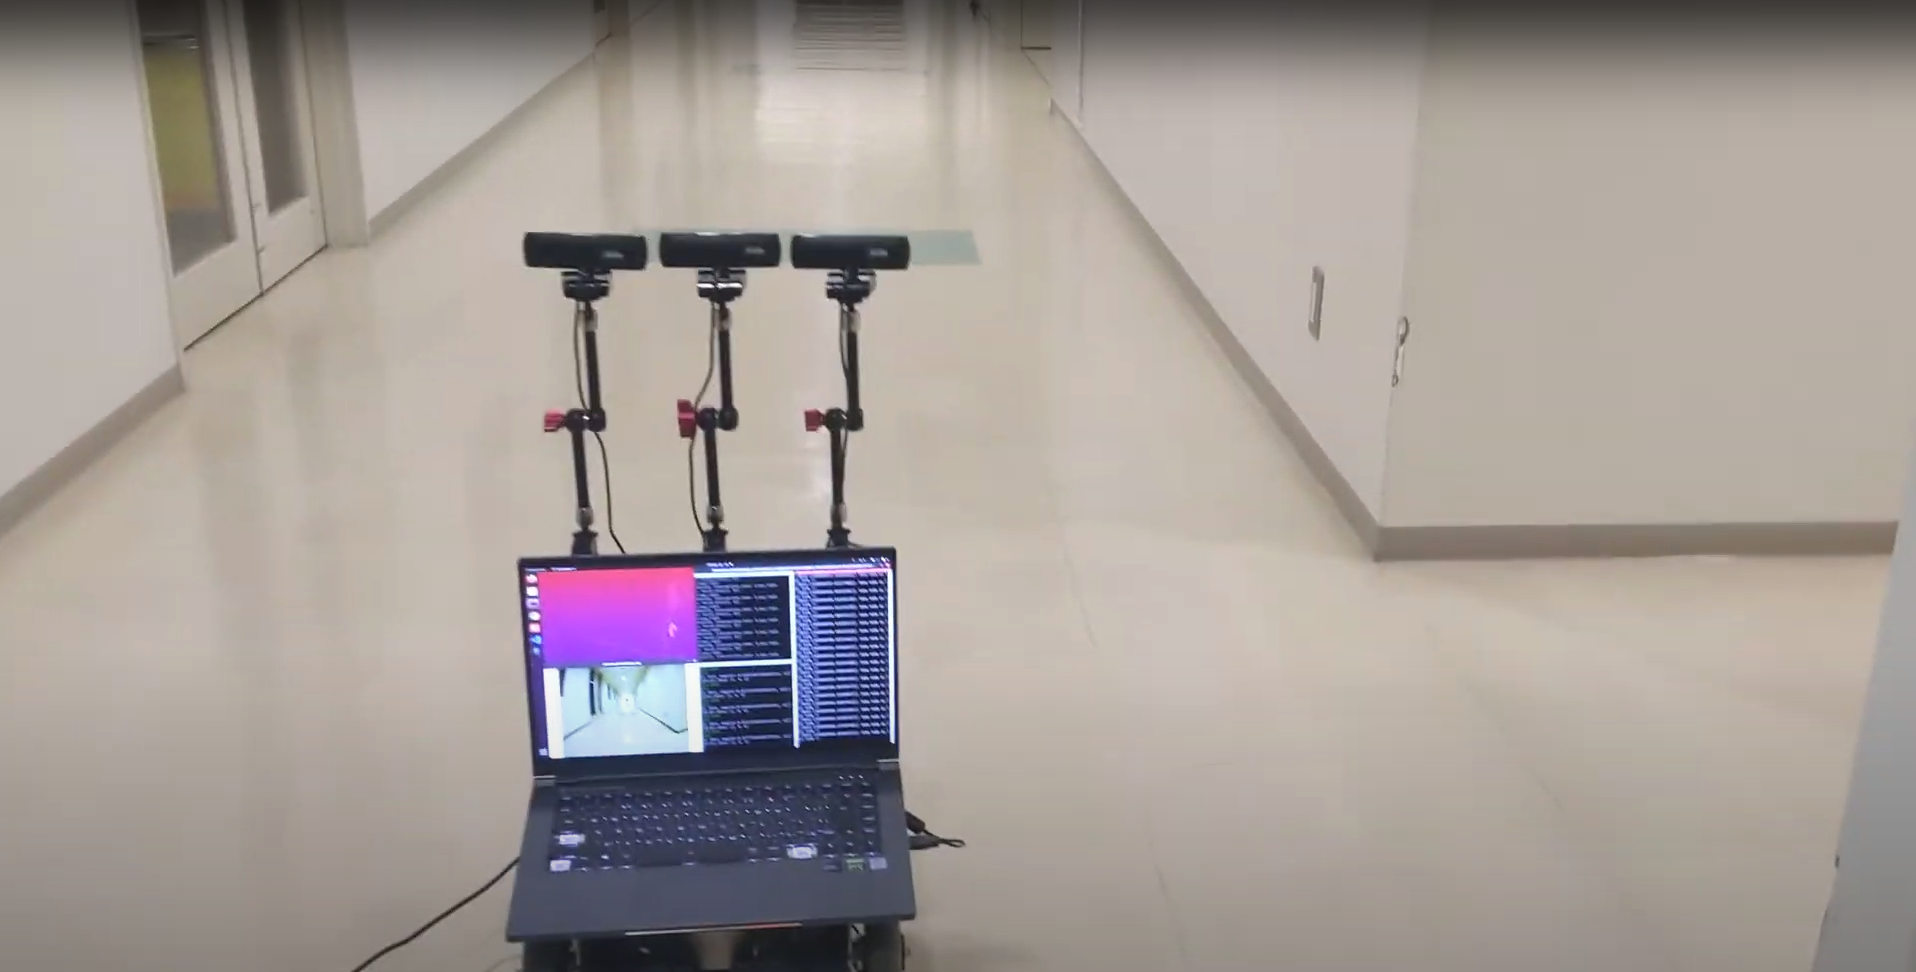
\includegraphics[keepaspectratio, width=80mm]{figs/exp_path_follow_0.png}
            \subcaption{3つ目の三叉路まで直進(First 3-way)}
        \end{minipage} &
        \begin{minipage}[t]{0.5\textwidth}
            \centering
            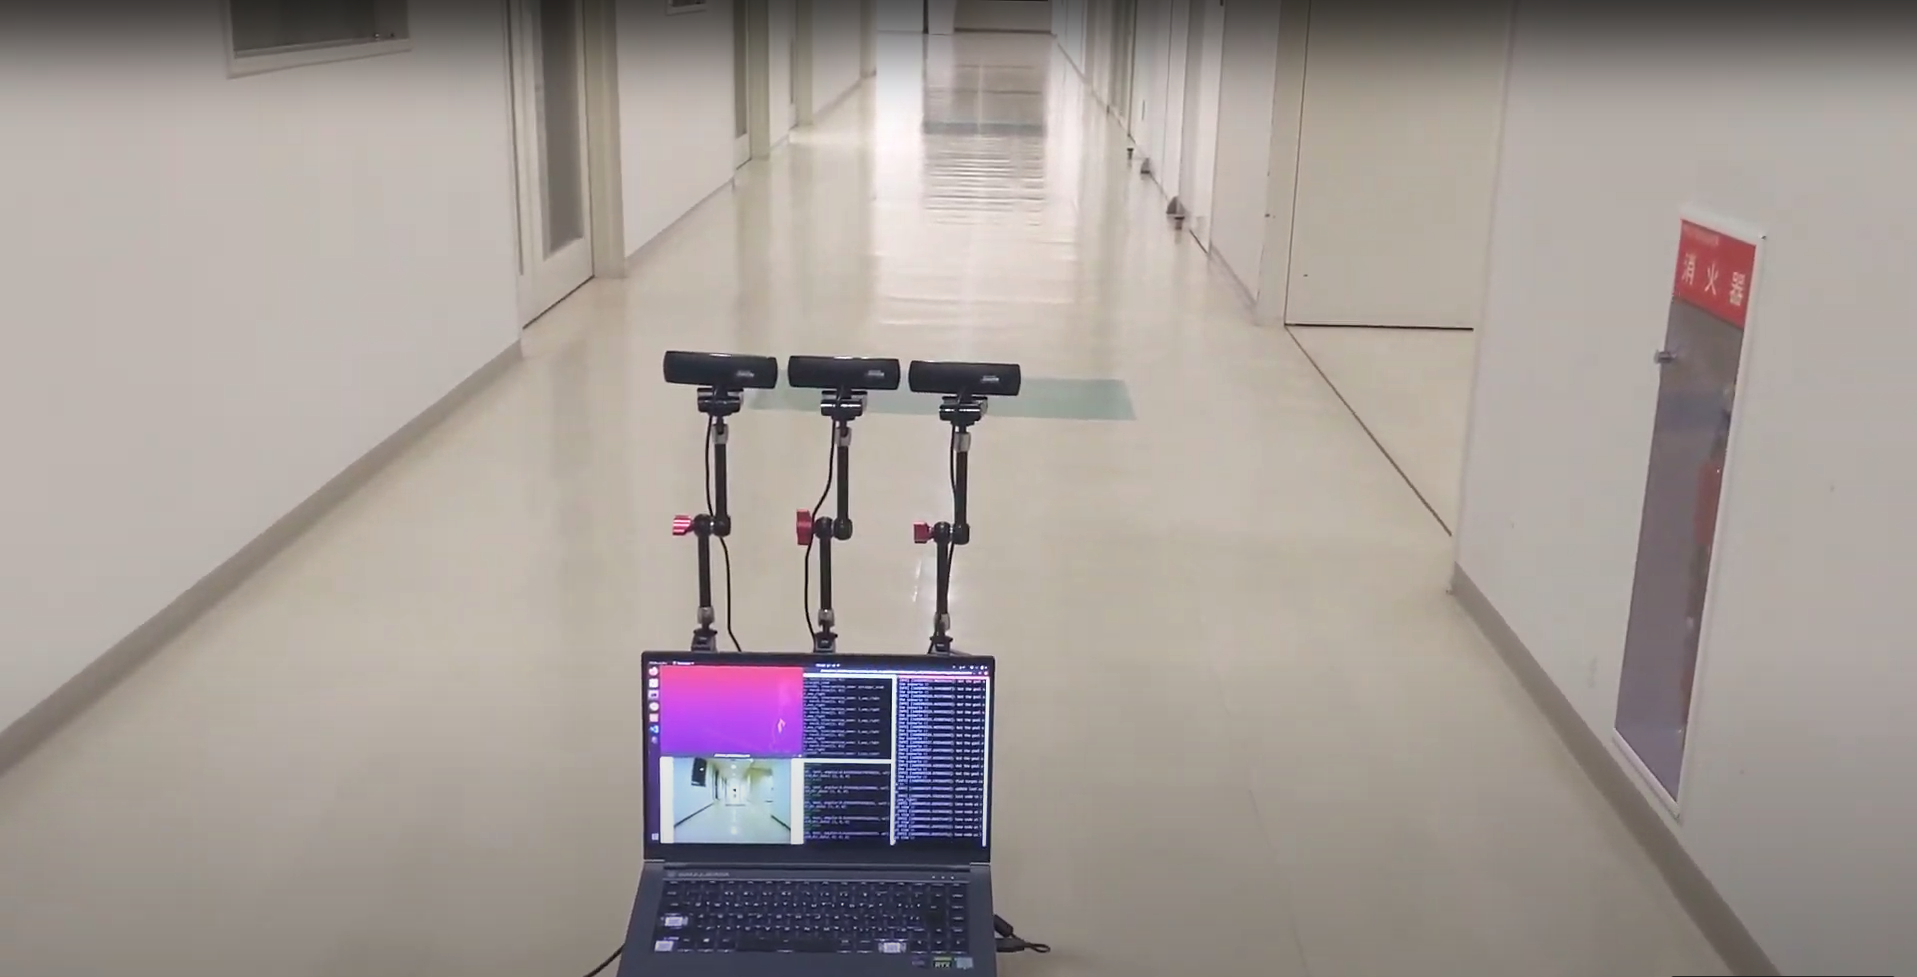
\includegraphics[keepaspectratio, width=80mm]{figs/exp_path_follow_1.png}
            \subcaption{3つ目の三叉路まで直進(Second 3-way)}
        \end{minipage} \\

        \begin{minipage}[t]{0.5\textwidth}
            \centering
            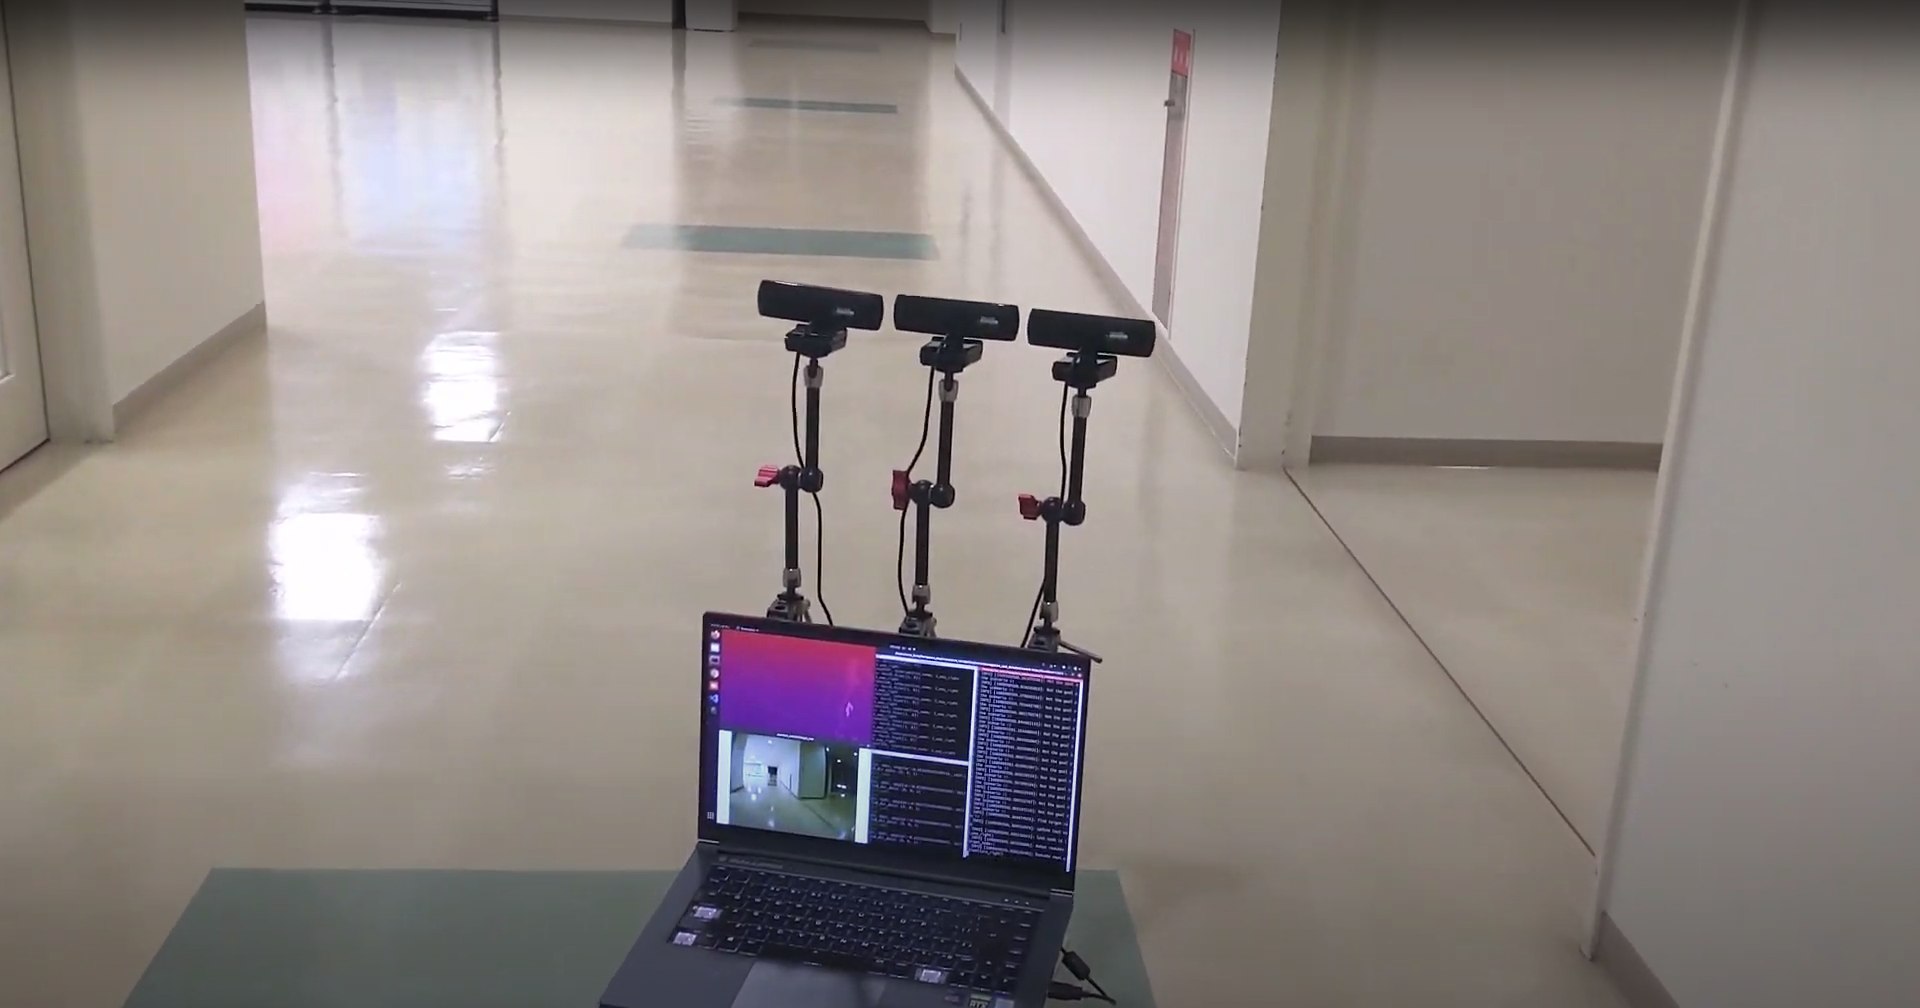
\includegraphics[keepaspectratio, width=80mm]{figs/exp_path_follow_2.png}
            \subcaption{右折(Third 3-way)}
        \end{minipage} &
        \begin{minipage}[t]{0.5\textwidth}
            \centering
            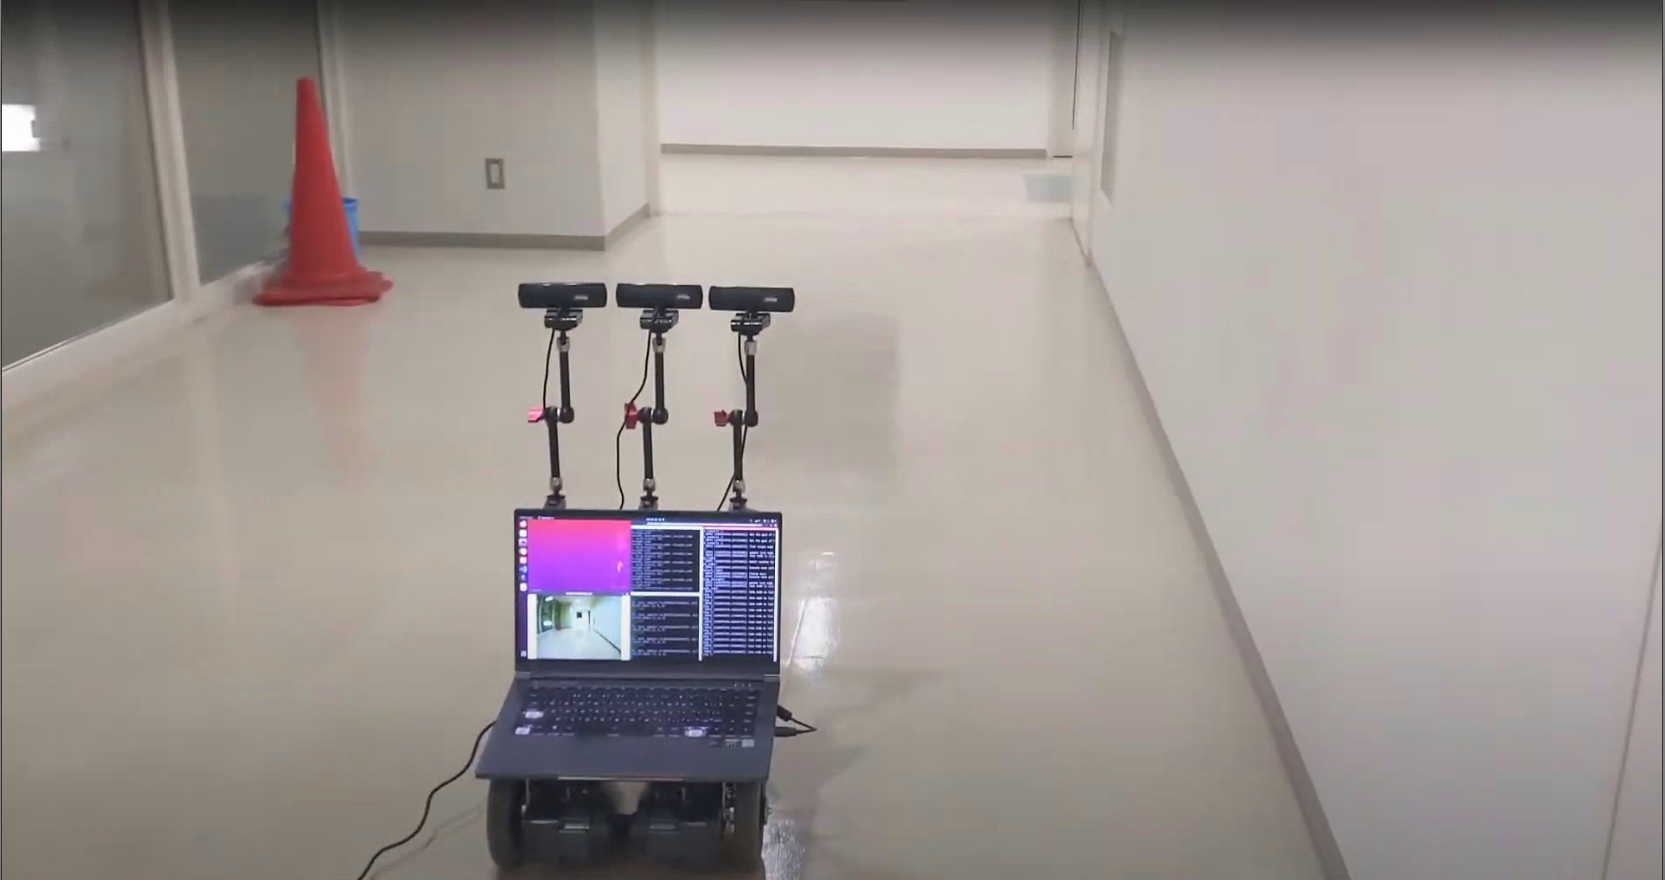
\includegraphics[keepaspectratio, width=80mm]{figs/exp_path_follow_4.png}
            \subcaption{突き当たりまで直進(Straight road)}
        \end{minipage} \\
        \begin{minipage}[t]{0.5\textwidth}
            \centering
            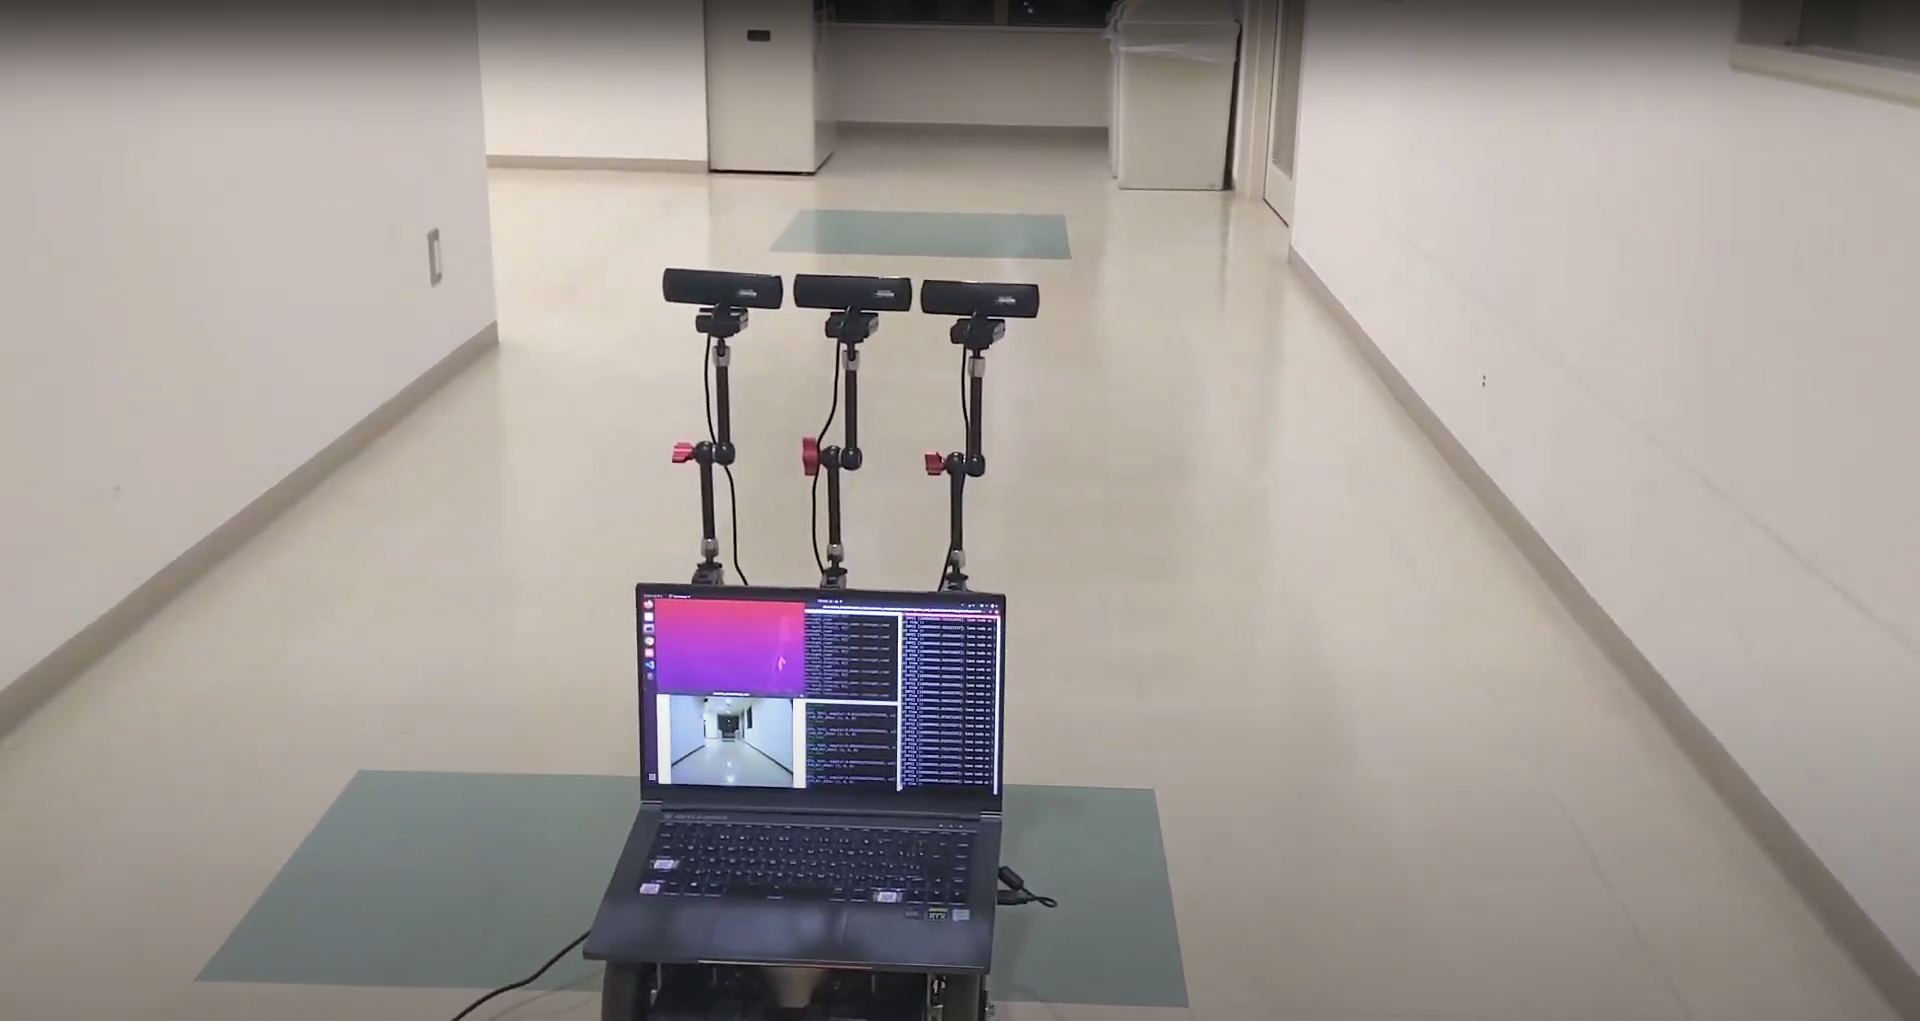
\includegraphics[keepaspectratio, width=80mm]{figs/exp_path_follow_5.png}
            \subcaption{左折(End)}
        \end{minipage} &
        \begin{minipage}[t]{0.5\textwidth}
            \centering
            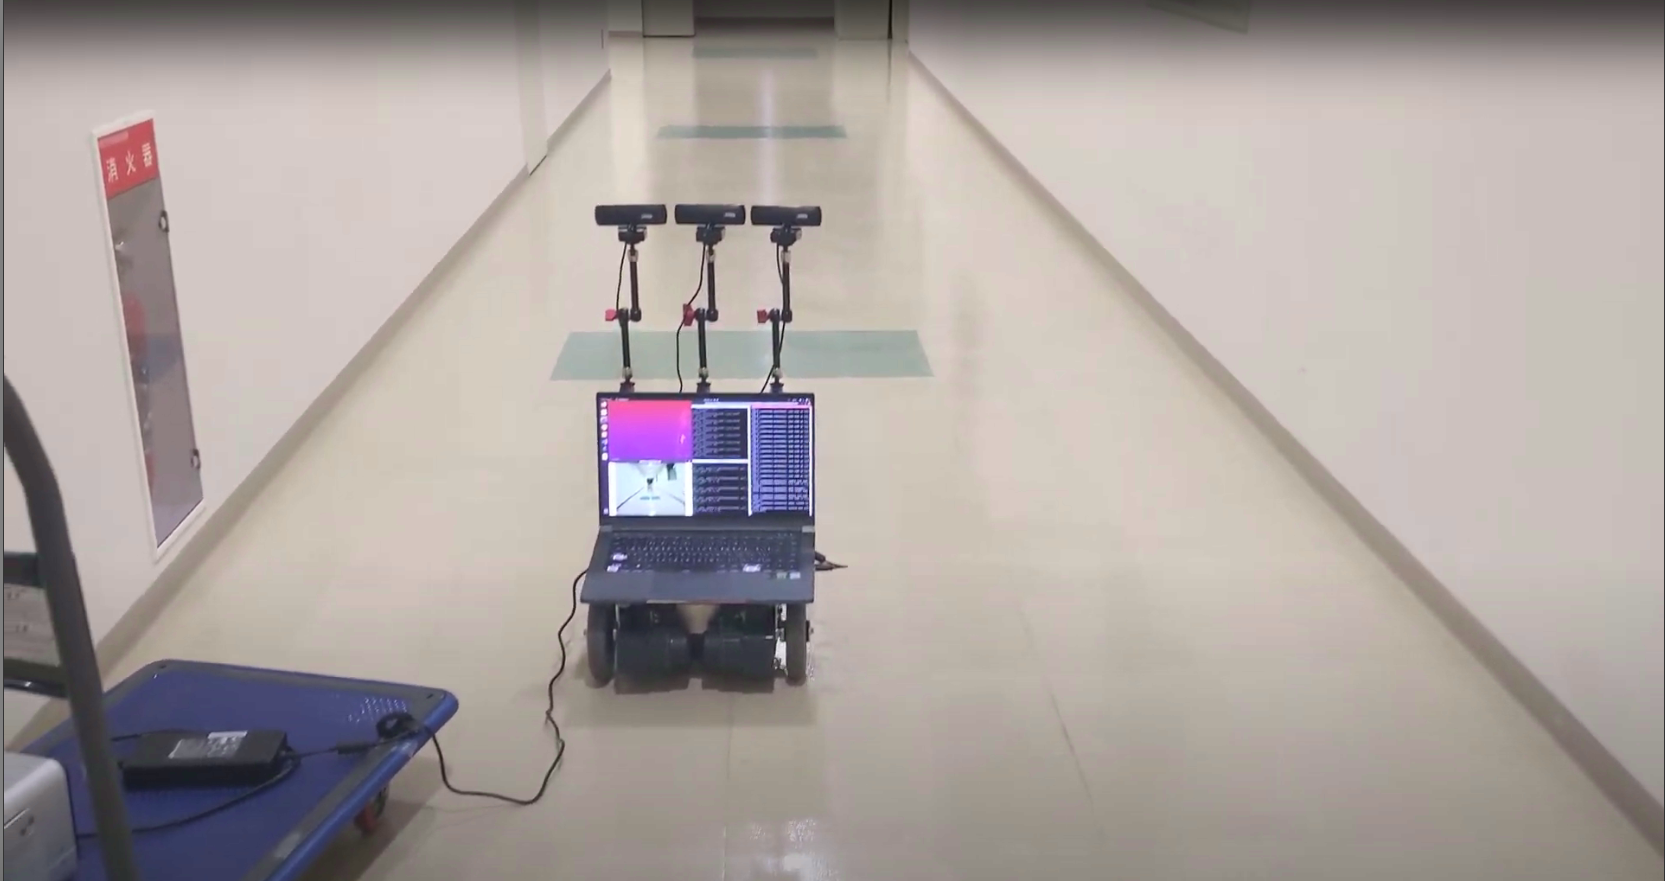
\includegraphics[keepaspectratio, width=80mm]{figs/exp_path_follow_6.png}
            \subcaption{突き当たりまで直進(Straight road)}
        \end{minipage} \\
        \begin{minipage}[t]{0.5\textwidth}
            \centering
            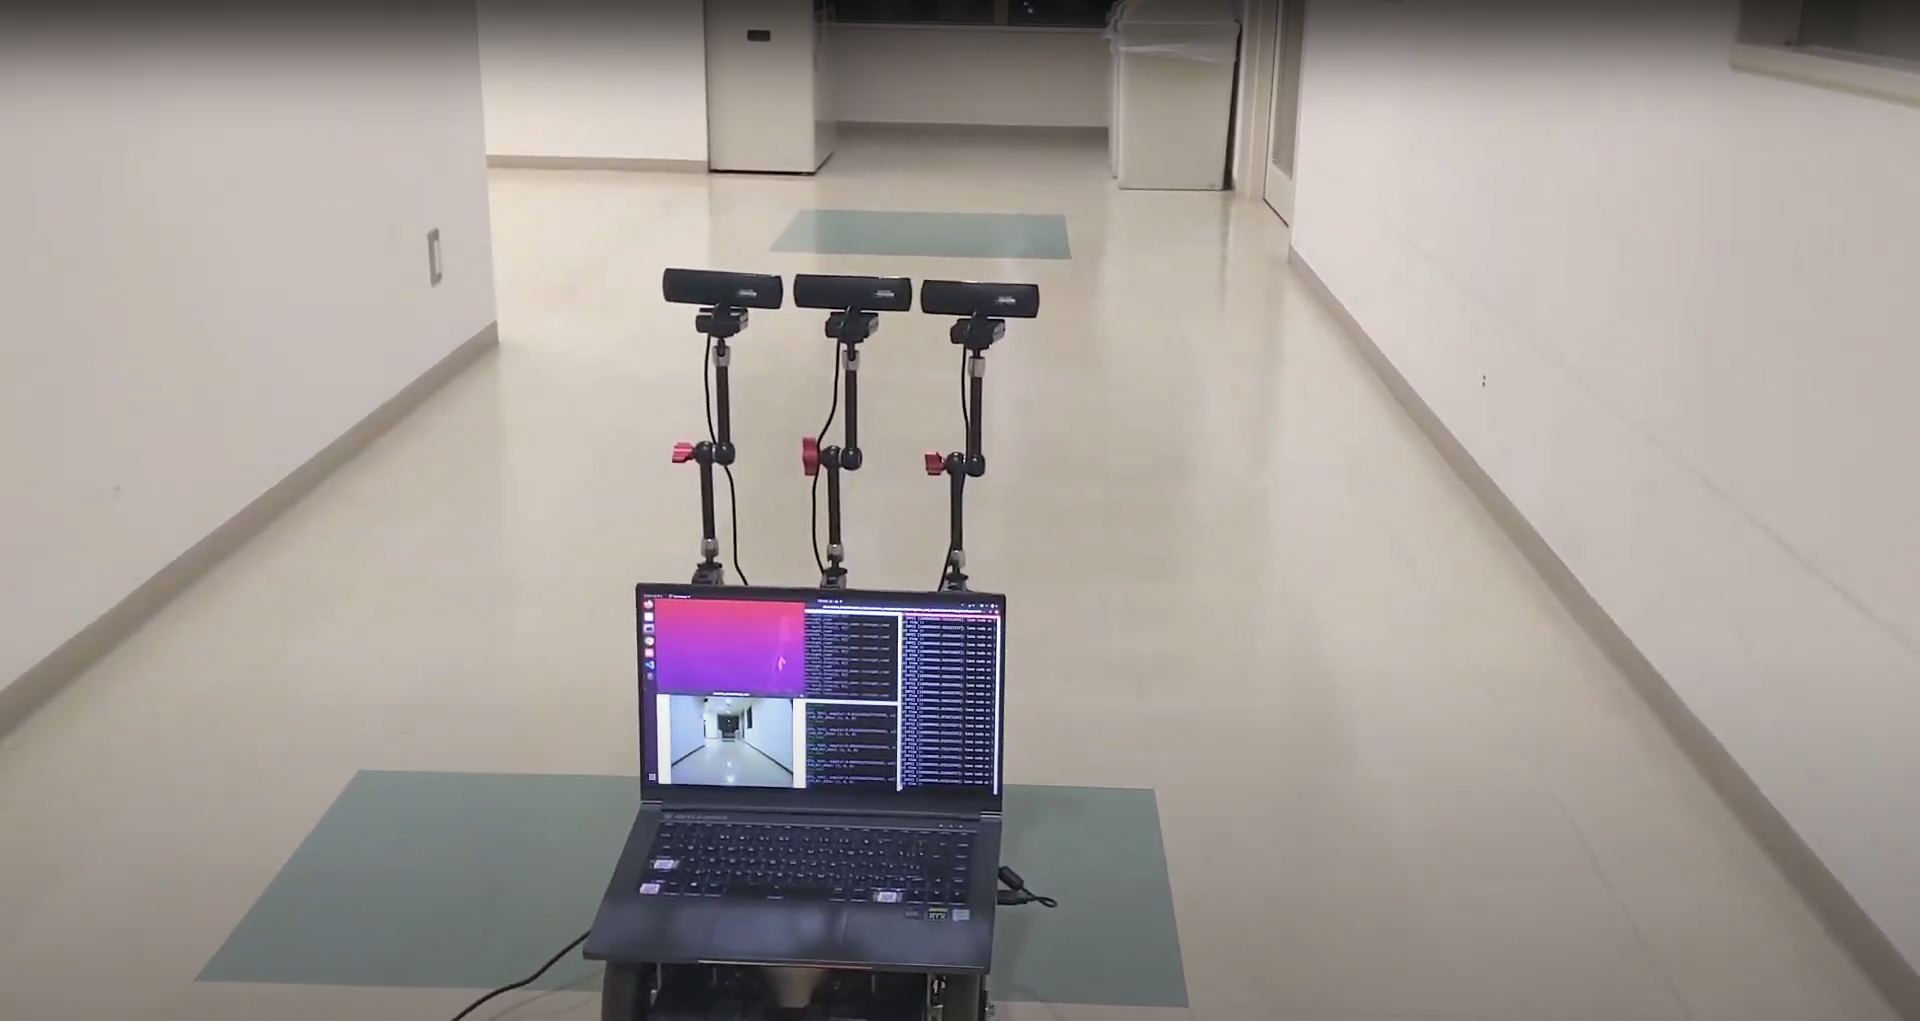
\includegraphics[keepaspectratio, width=80mm]{figs/exp_path_follow_7.png}
            \subcaption{停止(End)}
        \end{minipage}
    \end{tabular}

    \caption{An example of the robot applied the proposed system}\label{fig:exp_path}
\end{figure*}
% \begin{figure*}[htbp]\vspace*{-10zh}
%     \centering
%      \includegraphics[height=60mm,width=180mm]{./figs/exp_etc.png}
%      \caption{Behavior of path following in scenario24}\label{fig:exp}
% \end{figure*}
% \begin{table}[h!]
%     \centering
%     \caption{The number of assistances in the experiment}\label{tab:result}
%     % \begin{tabular}{ccclll}
        
%     % \begin{tabularx}{\textwidth}{X|X|X}
%     \begin{tabularx}{80mm}{|C|C|C|}
%     \hline
%     Scenario number used in the experiment & 
%     Number of assistances for deviating from the path & 
%     Number of assistances due to corridor classification failures \\
%     \hline
%     1       & 0         & 0             \\
%     5       & 0         & 0             \\
%     20      & 0         & 0             \\
%     21      & 0         & 0             \\
%     22      & 0         & 0             \\
%     24      & 0         & 0             \\
%     50      & 0         & 0             \\
%     \hline
%     % \end{tabular}
%     \end{tabularx}
%     \end{table}
\end{document}
